%% MemGate capstone project report ("black book"), SVKM's NMIMS STME Indore.
%% Format: Capstone project guidelines 2026-27, Annexure A.8, and the STME
%% front-matter template. Build with ./build.sh (pdflatex + bibtex).
%% Team details (names, SAP IDs, stream) are in details.tex.
\documentclass[12pt,a4paper,oneside]{report}

\usepackage[a4paper,left=1.5in,right=1in,top=1in,bottom=1in,headheight=15pt]{geometry}
\usepackage[T1]{fontenc}
\usepackage{mathptmx}   % Times New Roman (text and maths)
\usepackage{setspace}
\usepackage{titlesec}
\usepackage{fancyhdr}
\usepackage{graphicx}
\usepackage{booktabs}
\usepackage{adjustbox}
\usepackage{array}
\usepackage{tabularx}
\usepackage{longtable}
\usepackage{multirow}
\usepackage{enumitem}
\usepackage{caption}
\usepackage{amsmath,amssymb}
\usepackage{algorithm}
\usepackage{algpseudocode}
\usepackage{xcolor}
\usepackage{tikz}
\usetikzlibrary{arrows.meta,positioning,shapes.geometric,calc,fit}
\usepackage{pdfpages}
\usepackage{rotating}
\usepackage{cite}
\usepackage{url}
\usepackage[hidelinks]{hyperref}

%% Everything personal to the team lives here. Edit this file, then rebuild:
%%   cd report && ./build.sh
%% A field left as \blankfield{...} prints as a line to be filled by hand.
\newcommand{\blankfield}[1]{\underline{\hspace{#1}}}

\newcommand{\projtitle}{MemGate: An Adaptive Memory Layer for Long-Running LLM Agents}
\newcommand{\projtitleshort}{MemGate: Adaptive Memory for LLM Agents}
\newcommand{\paperTitle}{Selection Beats Compression: Memory Decision Policies for LLM Agents Under a Bounded Store}
\newcommand{\acadyear}{2026--27}

\newcommand{\studentA}{Yash Ramchandani}
\newcommand{\sapA}{70562300097}
\newcommand{\studentB}{Simar Singh Khanuja}
\newcommand{\sapB}{70562200088}

\newcommand{\mentor}{Dr.\ Praveen Modi}
\newcommand{\mentordesig}{Assistant Professor}

%% Program stream: the front matter template offers
%% "Artificial Intelligence and Data Science (AI\&DS)" or "Computer Engineering (CE)".
%% Not yet confirmed by the team, so it prints as a blank.
\newcommand{\stream}{\blankfield{7cm}}
\newcommand{\streamshort}{\blankfield{4cm}}

\newcommand{\assocdean}{Dr.\ Vikas Khare}
\newcommand{\director}{Dr.\ Anshuman Jaswal}


%% ---------------------------------------------------------------- layout
\onehalfspacing
\emergencystretch=3em
\setlength{\parskip}{4pt}
\setlist{itemsep=2pt,topsep=4pt}

% chapter title 18 pt bold, section 14 pt bold, subsection 12 pt bold
\titleformat{\chapter}[display]
  {\centering\bfseries\fontsize{18}{22}\selectfont}
  {\chaptertitlename\ \thechapter}{10pt}{\fontsize{18}{22}\selectfont}
\titleformat{name=\chapter,numberless}[display]
  {\centering\bfseries\fontsize{18}{22}\selectfont}{}{0pt}{\fontsize{18}{22}\selectfont}
\titlespacing*{\chapter}{0pt}{0pt}{20pt}
\titleformat{\section}{\bfseries\fontsize{14}{17}\selectfont}{\thesection}{0.6em}{}
\titleformat{\subsection}{\bfseries\fontsize{12}{15}\selectfont}{\thesubsection}{0.6em}{}
\titlespacing*{\section}{0pt}{14pt}{6pt}
\titlespacing*{\subsection}{0pt}{10pt}{4pt}

% figure names below figures, table names above tables, Times 10 pt
\DeclareCaptionFont{tenpt}{\fontsize{10}{12}\selectfont}
\captionsetup{font=tenpt,labelfont={tenpt,bf},labelsep=period,justification=centering}
\captionsetup[table]{position=top,skip=4pt}
\captionsetup[figure]{position=bottom,skip=6pt}

% header: project title left, academic year right; footer: page number right
\pagestyle{fancy}
\fancyhf{}
\fancyhead[L]{\fontsize{10}{12}\selectfont\projtitleshort}
\fancyhead[R]{\fontsize{10}{12}\selectfont Academic Year \acadyear}
\fancyfoot[R]{\thepage}
\renewcommand{\headrulewidth}{0.4pt}
\fancypagestyle{plain}{\fancyhf{}%
  \fancyhead[L]{\fontsize{10}{12}\selectfont\projtitleshort}%
  \fancyhead[R]{\fontsize{10}{12}\selectfont Academic Year \acadyear}%
  \fancyfoot[R]{\thepage}}

% the paper's diagrams and tables are reused as they are
\newcommand{\colfig}{0.8\textwidth}
\renewcommand{\listfigurename}{List of Figures}
\renewcommand{\listtablename}{List of Tables}
\renewcommand{\bibname}{References}

\begin{document}
% Shared TikZ styles for the hand-drawn diagrams (\input by main.tex).
\tikzset{
  >={Stealth[length=2mm]},
  box/.style={draw, rounded corners=2pt, align=center, fill=white,
              inner sep=3pt, font=\footnotesize},
  tier/.style={box, fill=blue!6, minimum height=7mm},
  proc/.style={box, fill=gray!8},
  model/.style={box, fill=orange!10},
  dec/.style={draw, diamond, aspect=2.2, align=center, inner sep=1pt,
              fill=yellow!10, font=\scriptsize},
  res/.style={box, fill=green!8, font=\scriptsize},
  bad/.style={box, fill=red!8, font=\scriptsize},
  lab/.style={font=\scriptsize, inner sep=1pt},
  flow/.style={->, thick},
  aux/.style={->, densely dashed},
}


%% ================================================================ title
\begin{titlepage}
\centering
\vspace*{0.2cm}
{\fontsize{18}{24}\selectfont\bfseries \projtitle\par}
\vspace{1.0cm}
{\large\bfseries Project Report submitted in partial fulfilment\\ of\par}
\vspace{0.4cm}
{\large Bachelor of Technology (B.Tech) in\par}
\vspace{0.2cm}
{\large \stream\par}
\vspace{0.8cm}
{\large\bfseries by\par}
\vspace{0.4cm}
{\large \textbf{\studentA} (SAP ID: \sapA)\\[2pt]
        \textbf{\studentB} (SAP ID: \sapB)\par}
\vspace{0.8cm}
{\large\bfseries Under the supervision of\par}
\vspace{0.4cm}
{\large\bfseries \mentor\par}
{(\mentordesig, STME, Indore Campus)\par}
\vfill
{\large\bfseries SVKM's NMIMS University\par}
{(Deemed-to-be University)\par}
\vspace{0.4cm}

\includegraphics[width=2.8cm]{images/nmims_logo.png}\par
\vspace{0.3cm}
{\large\bfseries SCHOOL OF TECHNOLOGY MANAGEMENT \&\\ ENGINEERING (STME)\par}
\vspace{0.3cm}
{\bfseries \acadyear\par}
\end{titlepage}

%% ========================================================== certificate
\thispagestyle{empty}
\begin{center}
{\fontsize{18}{22}\selectfont\bfseries CERTIFICATE\par}
\vspace{0.6cm}

\includegraphics[width=3cm]{images/nmims_logo.png}\par
\vspace{0.4cm}
{\large\bfseries SVKM's NMIMS University\\ (Deemed-to-be University)\par}
\end{center}
\vspace{0.4cm}
\noindent This is to certify that the project entitled \textbf{``\projtitle''}
has been done by \textbf{\studentA} (SAP: \sapA) and \textbf{\studentB}
(SAP: \sapB) under my guidance and supervision \& has been submitted in partial
fulfilment of the degree of \textbf{B.Tech} in \textbf{\streamshort} of STME,
SVKM's NMIMS (Deemed-to-be University), Indore Campus, India.

\vspace{2.2cm}
\noindent\rule{5cm}{0.4pt}\\
\textbf{\mentor}\\
(Internal Guide)

\vspace{1.8cm}
\noindent\rule{5cm}{0.4pt}\\
\textbf{Examiner}\\
(External)

\vspace{1.8cm}
\noindent\rule{5cm}{0.4pt}\\
\textbf{\assocdean}\\
(Associate Dean, STME)

\vfill
\noindent\textbf{Date:} \rule{3cm}{0.4pt}\hfill\textbf{Place:} Indore
\clearpage

%% ======================================================== roman numbers
\pagenumbering{roman}
\setcounter{page}{1}

\chapter*{Acknowledgement}
\addcontentsline{toc}{chapter}{Acknowledgement}
We would like to express our sincere gratitude to all those who contributed to
the successful completion of this project.

First and foremost, we extend our heartfelt thanks to our faculty mentor,
\textbf{\mentor}, \mentordesig, for invaluable guidance, continuous
support and insightful feedback throughout the course of this project. The
mentor's review of our research paper, and the steady push for every claim to
be backed by a measurement, shaped this work.

We are deeply grateful to SVKM's NMIMS University and the School of Technology
Management \& Engineering (STME) for providing the necessary resources,
infrastructure and academic environment that made this work possible.

We would like to express our profound gratitude to \textbf{\director},
Director, NMIMS University Indore Campus. We also extend our sincere thanks to
\textbf{\assocdean}, Associate Dean, School of Technology Management \&
Engineering (STME), Indore Campus, for his continuous support and motivation.

We would also like to thank the faculty members of STME for their teaching and
support, which laid the foundation for this project, and the members of the
review panels, whose questions at Review~1 led us to move the project's
contribution from the memory architecture to the memory decision policy.

We thank the authors of the LoCoMo, REALTALK, BEAM, MemBench, PersonaChat and
LongMemEval datasets for releasing them openly; this project collected no data
of its own.

Finally, we are immensely thankful to our families for their unwavering
support, patience and encouragement throughout our academic journey.

\vspace{1.2cm}
\begin{flushright}
\textbf{\studentA} (SAP: \sapA)\\
\textbf{\studentB} (SAP: \sapB)
\end{flushright}

\chapter*{Abstract}
\addcontentsline{toc}{chapter}{Abstract}
Agents built on large language models (LLMs) now hold conversations that run
for weeks and grow far longer than any context window. On every turn something
has to decide which parts of that history go into the prompt. Re-sending the
whole history makes each reply slower and costlier, a sliding window forgets
the oldest messages whatever they contain, and uniform summarisation loses the
names, numbers and dates that are asked about later. Existing memory systems combine tiers, summaries and forgetting,
but they are evaluated end to end, so the value of each individual decision is
unknown.

This project builds \textbf{MemGate}, a memory layer that sits between an
agent and a frozen LLM and decides, for every message, whether to
\emph{keep} it, \emph{compress} it, \emph{forget} it, or \emph{recall} it
later, without training the base model. It is built as a measurement
harness: a three-tier store runs under a fixed storage budget, and policies
that differ in exactly one factor are compared on the LoCoMo benchmark with
95\% confidence intervals resampled by conversation.

The main findings are as follows. (i) The usual accounting bounds the
context but not the store; once the store is bounded, choosing
\emph{which} turns to forget gains $+9.37$ answer-recall points over
oldest-first eviction at identical storage, fidelity and retrieval, while
compressing evicted turns instead of dropping them loses $7.13$ points.
(ii) No rate--distortion crossover appears up to $182\times$ compression.
(iii) Counting the embedding index in bytes reverses the ranking below about
40\,KiB. (iv) A small LLM judge of salience loses to a hand-written heuristic,
whereas a logistic-regression scorer over shallow features and a sentence
embedding, trained on generated and human conversations, beats the heuristic
by $+14.55$ points on held-out conversations and outperforms rebuilt
MemGPT-style and Mem0-style memory at every budget tested. (v) On held-out
chats of up to ten million tokens it beats retrieval on every corpus, and when
million-token chats are typed into the application it keeps the answer for
51.9\% of questions against 19.2\% for retrieval.

The learned scorer ships in a working chat application that shows, for every
message, the tier it went to and why. The work has been written up as a
research paper with the project mentor as corresponding author.

\vspace{6pt}
\noindent\textbf{Keywords:} large language models, agent memory, context
management, retrieval-augmented generation, learned salience scoring,
rate--distortion, empirical evaluation.


\tableofcontents
\clearpage
\phantomsection
\addcontentsline{toc}{chapter}{List of Figures}
\listoffigures
\clearpage
\phantomsection
\addcontentsline{toc}{chapter}{List of Tables}
\listoftables
\clearpage
\chapter*{Abbreviations}
\addcontentsline{toc}{chapter}{Abbreviations}
\begin{center}
\setstretch{1.1}
\begin{longtable}{@{}p{3.2cm}p{10.5cm}@{}}
\toprule
\textbf{Abbreviation} & \textbf{Full form} \\
\midrule
\endhead
API & Application Programming Interface \\
AUC & Area Under the (ROC) Curve \\
BEAM & Benchmark for long-context memory (100K to 10M-token chats) \\
CI & Confidence Interval \\
CPU / GPU & Central / Graphics Processing Unit \\
F1 & Harmonic mean of precision and recall \\
FIFO & First In, First Out \\
JSON & JavaScript Object Notation \\
KiB & Kibibyte (1{,}024 bytes) \\
KV cache & Key--Value cache of a transformer's attention \\
LLM & Large Language Model \\
LoCoMo & Long Conversational Memory benchmark \\
LOCO & Leave-One-Conversation-Out (cross-validation) \\
LR & Logistic Regression \\
MiniLM & all-MiniLM-L6-v2 sentence embedding model \\
MLP & Multi-Layer Perceptron \\
NER & Named-Entity Recognition \\
n.s. & not significant \\
ONNX & Open Neural Network Exchange (model format) \\
P0 & Sliding-window policy (recency only) \\
P1 & MemGate with the hand-written heuristic scorer \\
P1-A & MemGate, adaptive mode: compress on eviction \\
P1-S & MemGate, select mode: drop on eviction \\
P2 & MemGate with an LLM judge as scorer \\
P3 & MemGate with the learned (logistic) scorer \\
PDF & Portable Document Format \\
QA & Question Answering \\
RAG & Retrieval-Augmented Generation (store-all, FIFO baseline) \\
REST & Representational State Transfer (web API style) \\
$S$ & Storage budget of the memory store \\
$B$ & Context budget of the assembled prompt \\
UI & User Interface \\
UTF-8 & Unicode Transformation Format, 8-bit \\
\bottomrule
\end{longtable}
\end{center}


%% ======================================================= decimal numbers
\clearpage
\pagenumbering{arabic}
\setcounter{page}{1}

\chapter{Introduction}
\label{ch:intro}

This chapter introduces the problem that MemGate addresses: how a long-running
agent built on a large language model should decide what to remember. It
explains why larger context windows do not remove the need for that decision,
sets out the motivation and scope of the project, states the problem
precisely, lists the contributions, and describes how the rest of the report
is organised.

\section{Background of the project topic}

Large language models (LLMs) are now used as the core of \emph{agents}:
programs that plan, call tools, reflect on their own mistakes and carry on
working over many sessions
\cite{yao2023react,shinn2023reflexion,wang2024agentsurvey,xi2023agentsurvey}.
Coding assistants, research assistants, tutoring systems and personal
assistants are all expected to remember what was said days or weeks earlier.
An LLM, however, has no memory of its own between calls. Everything it knows
about the conversation has to be placed in its prompt, inside a fixed
\emph{context window} \cite{brown2020gpt3}.

The simplest way to give an agent memory is to append every message to a
growing prompt and send the whole history back to the model on every turn.
This works at first but does not scale. The cost of self-attention grows with
the square of the sequence length, and the key--value (KV) cache that the
model keeps grows with every token, so each reply becomes slower and more
expensive until the history no longer fits at all. Techniques that stretch the
window, such as position interpolation \cite{peng2024yarn}, delay that point
but do not remove it.

A larger window does not solve the quality problem either. Across frontier
models, accuracy drops by 30--50\% well before the advertised limit
\cite{chroma2025contextrot}; synthetic tests find effective context lengths
far shorter than the claimed ones \cite{hsieh2024ruler}; and how much a model
uses a passage depends on where it sits in a long input
\cite{liu2024lostmiddle}. These effects come from attention over long
sequences rather than from missing training data. What limits an agent is
therefore \emph{curation}, the choice of what goes into the prompt, rather than
raw capacity.

Several systems already manage agent memory. MemGPT \cite{packer2023memgpt}
pages a virtual context in and out of external storage, MemoryBank
\cite{zhong2024memorybank} applies a forgetting curve, Generative Agents
\cite{park2023generative} rank memories by recency, importance and relevance,
and Mem0 \cite{chhikara2025mem0} extracts and updates facts with an LLM.
Retrieval-augmented generation (RAG) \cite{lewis2020rag} stores everything and
retrieves the passages most similar to the query. Agent architectures now
treat memory as a module in its own right \cite{sumers2024coala}. These
designs show that tiered memory with forgetting works in practice. They are,
however, evaluated as complete systems, so it is not known how much each
individual decision inside them (what to keep, what to compress, what to
forget) is actually worth.

\section{Motivation and scope of the report}

\subsection{Motivation}
Poor curation has a measurable price. On the LongMemEval benchmark, a model
given oracle retrieval of the right evidence reaches about 92\% accuracy, while
the same model choosing its own evidence reaches about 58\%
\cite{wu2024longmemeval}. Given the right evidence the model answers
correctly, so the 34-point gap is a failure of \emph{selection}, not of
reasoning. A recent survey of agent memory puts it plainly: current systems
``do not solve the fundamental challenge: deciding what to remember and what
to forget'' \cite{zhang2024memorysurvey}. A rate--distortion view of these
decisions \cite{shannon1959rd,cover2006elements} has been proposed
\cite{colaco2026rd}, but as an analytical framework rather than a measured
system.

At Review~1 the panel asked whether a three-tier memory layer was still novel,
since commercial systems already ship one. The honest answer was that it is
not. The project therefore moved its contribution one level deeper, to the
\emph{decision policy} itself: building a layer in which each decision can be
isolated, swapped and measured, and then using it to find out which parts of
the familiar design actually earn their cost.

\subsection{Scope}
\textbf{In scope.}
\begin{itemize}
\item A memory controller that scores, compresses, stores, forgets and
  retrieves conversational memory in front of a frozen LLM, which is treated
  as a black box and never trained or fine-tuned.
\item A three-tier store (recent verbatim turns, compressed gists, durable
  facts with embeddings) held under a fixed storage budget.
\item Several interchangeable scoring policies: recency only, a hand-written
  heuristic, an LLM judge, and a learned scorer.
\item Evaluation on public long-conversation benchmarks (LoCoMo, REALTALK,
  BEAM, MemBench, PersonaChat, LongMemEval) with statistical tests that
  respect the clustering of questions by conversation.
\item A working chat application built on the same code, so that the memory
  decisions can be seen and tested by a user.
\end{itemize}

\textbf{Out of scope.} Training or fine-tuning the base LLM; image and audio
memory (the project is text only); production multi-user serving with
accounts and billing.

\section{Problem statement}

\begin{quote}
\emph{Given a conversation that grows without bound, a frozen LLM that can
only see a bounded context of $B$ tokens, and a memory store that may hold at
most $S$ tokens (or bytes), design and evaluate a memory decision policy that
chooses, for every message, whether to keep it verbatim, compress it, forget
it or recall it, so that the answers to later questions reach the model as
often as possible. Measure the contribution of each decision separately,
against controls that differ from it in exactly one factor.}
\end{quote}

The problem has two parts. The \emph{engineering} part is to build the layer
so that it is fast, never exceeds its budget, and works on real input. The
\emph{research} part is to find out, with proper statistics, whether
scored forgetting beats oldest-first forgetting, whether compressing beats
dropping, whether a learned scorer beats a hand-written one, and whether the
answer survives a change of corpus.

\section{Salient contribution}

The project makes the following contributions.
\begin{enumerate}
\item \textbf{A storage-budgeted evaluation protocol.} Bounding only the
  assembled context charges a store-everything baseline nothing for what it
  keeps. MemGate bounds the whole store, which changes the ranking of the
  policies (Section~\ref{sec:accounting}).
\item \textbf{Selection pays; compression does not.} At identical storage,
  fidelity and retrieval, scored forgetting gains $+9.37$ answer-recall points
  over FIFO, while compressing an evicted turn instead of dropping it costs
  $7.13$ points (Sections~\ref{sec:selection} and~\ref{sec:significance}).
\item \textbf{A test of the rate--distortion crossover} up to $182\times$
  compression, which is not reached (Section~\ref{sec:scaling}).
\item \textbf{Byte accounting.} The embedding index outweighs the text it
  indexes by about $12\times$ and reverses the policy ranking below roughly
  40\,KiB (Section~\ref{sec:bytes}).
\item \textbf{A negative result for LLM-judged salience.} A 0.5B judge loses
  to a hand-written heuristic by $5.87$ points (Section~\ref{sec:scorer}).
\item \textbf{A learned scorer} trained on generated and human conversations,
  with the direction in which it transfers and the one in which it does not
  (Section~\ref{sec:transfer}).
\item \textbf{End-task accuracy} through a fixed reader, showing how much of
  the recall advantage becomes correct answers (Section~\ref{sec:endtask}).
\item \textbf{Comparison with MemGPT-style and Mem0-style memory} rebuilt in
  the same harness (Section~\ref{sec:external}).
\item \textbf{Scale.} A test on chats of up to ten million tokens and a scorer
  retrained on 14.6 times the data (Sections~\ref{sec:scale}
  and~\ref{sec:retrain}).
\item \textbf{A working application.} A chat app that runs the shipped scorer,
  shows every keep, compress and forget decision with its reasons, accepts
  pasted text and uploaded documents, and was stress-tested on million-token
  chats and 200 simultaneous users (Sections~\ref{sec:app}
  and~\ref{sec:stress}).
\item \textbf{A research paper}, ``\paperTitle'', prepared in conference and
  journal versions.
\end{enumerate}

Several of these results are negative or corrective. We regard that as the
useful part: described only as a three-tier memory layer, MemGate would repeat
work others have done, whereas measured against controls it shows which parts
of that design are worth their cost.

\section{Organisation of report}

The rest of the report is organised as follows.
\textbf{Chapter~\ref{ch:lit}} surveys the literature on agent memory, prompt
and cache compression, retrieval and evaluation, compares the main systems,
and identifies the research gap.
\textbf{Chapter~\ref{ch:method}} describes the methodology and implementation:
the block diagram, the computing resources used, the scoring, routing and
budget algorithms with their equations and flowcharts, the training of the
learned scorer, the experimental design, and the chat application.
\textbf{Chapter~\ref{ch:results}} presents the results and their analysis,
with confidence intervals, together with the standards followed.
\textbf{Chapter~\ref{ch:adv}} discusses advantages, limitations and
applications, and \textbf{Chapter~\ref{ch:concl}} concludes and sets out the
future scope. The appendices contain the flowcharts of the software, data
sheets of the datasets and models, the list of software components, and the
papers prepared from this work.

\section*{Summary}
LLM agents need a policy that decides what to remember, because larger
context windows move the problem rather than remove it. Existing memory
systems are evaluated whole, so the worth of each decision is unknown. MemGate
is built to measure those decisions one at a time under a bounded store, and
the rest of this report describes how it was built and what it found.

\chapter{Literature Survey}
\label{ch:lit}

This chapter reviews the work on which MemGate builds. It first gives the
background of the overall topic: why LLM agents need memory, how long
contexts fail, and the older ideas from computer systems and psychology that
memory layers borrow. It then surveys the most relevant papers one by one,
compares them in a table, and ends by identifying the research gap that
defines the problem addressed in this project.

\section{Introduction to the overall topic}

\subsection{LLM agents and their memory}
Large language models learn to perform new tasks from instructions and a few
examples placed in the prompt \cite{brown2020gpt3}. Building on this, agent
frameworks interleave reasoning with actions such as tool calls
\cite{yao2023react} and let a model learn from its own failures by writing
verbal reflections into its context \cite{shinn2023reflexion}. Two broad
surveys describe how such agents are assembled from a profile, a planner, a
memory and an action module
\cite{wang2024agentsurvey,xi2023agentsurvey}, and the CoALA framework treats
memory explicitly as working, episodic, semantic and procedural stores around
the model \cite{sumers2024coala}. A survey devoted to agent memory organises
the field by memory source, form and operation, and concludes that deciding
what to remember and what to forget remains the open problem
\cite{zhang2024memorysurvey}.

\subsection{Why longer context windows are not enough}
One response is to make the window larger. YaRN extends the context of
existing models by interpolating rotary position embeddings
\cite{peng2024yarn}. Larger windows, however, are used unevenly. Models make
best use of information at the beginning and the end of a long input and
lose it in the middle \cite{liu2024lostmiddle}; the RULER benchmark finds
effective context lengths far below the advertised ones \cite{hsieh2024ruler};
and a 2025 study of 18 frontier models reports accuracy losses of 30--50\% well
before the documented limit \cite{chroma2025contextrot}. Long-context
benchmarks such as LongBench measure this capacity directly, without a memory
layer \cite{bai2024longbench}.

\subsection{Retrieval as the default baseline}
Retrieval-augmented generation (RAG) keeps external text and puts the passages
most similar to the query into the prompt \cite{lewis2020rag}. Dense passage
retrieval made this practical with learned sentence embeddings
\cite{karpukhin2020dpr}, and RETRO showed that retrieval from a very large
store can stand in for model size \cite{borgeaud2022retro}. Sentence-BERT
\cite{reimers2019sbert} and the distilled MiniLM model \cite{wang2020minilm}
provide the small, fast embeddings that this project uses. RAG stores
everything and never forgets, so it is the natural control against which a
forgetting policy must be judged.

\subsection{Ideas borrowed from systems and psychology}
Memory layers for agents reuse older ideas. The multi-store model of human
memory separates a short-term store from a long-term store with control
processes between them \cite{atkinson1968memory}. Operating systems face the
same choice when physical memory is full: Belady's study of page replacement
\cite{belady1966replacement} and Denning's working-set model
\cite{denning1968workingset} are the classical treatments, and MemGPT makes
the analogy explicit \cite{packer2023memgpt}. Rate--distortion theory
\cite{shannon1959rd,cover2006elements} gives the language for trading the size
of a stored representation against its fidelity, and has recently been
proposed as a framework for agent memory \cite{colaco2026rd}.

\subsection{How memory is evaluated}
LoCoMo provides very long multi-session dialogues with question--answer pairs
whose evidence turns are marked \cite{maharana2024locomo}. LongMemEval
separates several abilities of chat assistants over long histories and
measures the gap between oracle and self-selected evidence
\cite{wu2024longmemeval}. REALTALK applies LoCoMo's annotation scheme to 21 days
of real messages between people \cite{lee2025realtalk}; BEAM scales
conversations to ten million tokens \cite{tavakoli2026beam}; and MemBench
tests factual and reflective memory of agents \cite{tan2025membench}.
LLM-as-a-judge evaluation \cite{zheng2023judge} is widely used for open-ended
answers, while extractive question answering is scored by string match
\cite{rajpurkar2016squad}. For comparing two systems on the same questions,
McNemar's test \cite{mcnemar1947,dietterich1998tests} and the bootstrap
\cite{efron1993bootstrap} are standard; when questions are grouped into
conversations, the resampling must respect that grouping
\cite{cameron2008cluster}. Finally, studies of data leakage show how easily an
evaluation can be contaminated by information that would not be available at
prediction time \cite{kaufman2012leakage,kapoor2023leakage}, a failure this
project met and fixed (Section~\ref{sec:leak}).

\section{Survey of the most relevant work}

This section discusses the most relevant papers in more detail, grouped by
the decision they make.

\subsection{Memory systems for agents}

\textbf{MemGPT} (Packer et al., 2023) \cite{packer2023memgpt} treats the
context window like the main memory of an operating system. The model itself
decides, through function calls, what to page out to an archive and what to
bring back, and a recursive summary keeps a compressed record of evicted
messages. MemGPT shows that an agent can work well beyond its window, and it
was chosen as the base paper of this project. Its limitation, for our
purpose, is that every memory decision is left to the LLM, so there is no
explicit importance policy whose value can be measured on its own.

\textbf{MemoryBank} (Zhong et al., 2024) \cite{zhong2024memorybank} adds a
long-term memory with an Ebbinghaus-style forgetting curve: memories decay
with elapsed time and are reinforced when recalled. It produces human-like
forgetting, but it forgets by age rather than by importance and does not hold
the store to a fixed budget.

\textbf{Generative Agents} (Park et al., 2023) \cite{park2023generative}
record a stream of observations for each simulated character and retrieve
from it by a weighted sum of recency, importance (rated by the LLM) and
relevance, with periodic reflections that summarise the stream. The design
sustains believable long-horizon behaviour, but the stream is never bounded
and the system is not built to reduce tokens or cost.

\textbf{A-MEM} (Xu et al., 2025) \cite{xu2025amem} organises memories as
linked notes in the style of a Zettelkasten. Each new memory is written as a
structured note, linked to related notes, and may cause older notes to be
revised. On LoCoMo it improves multi-hop reasoning while using fewer tokens.
Its focus is on how notes are linked rather than on what to forget under a
strict budget.

\textbf{Mem0} (Chhikara et al., 2025) \cite{chhikara2025mem0} is a
production-oriented memory layer. An LLM extracts candidate facts from each
exchange and chooses among ADD, UPDATE, DELETE and NOOP against the nearest
stored facts. It reports large savings in latency and tokens against
full-context baselines on LoCoMo. Because the extraction and update decisions
are made by an LLM end to end, the contribution of each decision cannot be
separated, which is why Section~\ref{sec:external} rebuilds its memory
structure inside the MemGate harness.

\subsection{Compressing the prompt or the cache}

\textbf{LLMLingua} (Jiang et al., 2023) \cite{jiang2023llmlingua} compresses a
given prompt by removing tokens that a small language model finds predictable,
under a budget controller, reaching up to about 20$\times$ compression with
small losses. It compresses what it is given but does not decide what to
store or forget across sessions.

\textbf{Gist tokens} (Mu et al., 2023) \cite{mu2023gist} train a model to
compress an instruction into a few virtual tokens that can be cached and
reused. \textbf{AutoCompressors} (Chevalier et al., 2023)
\cite{chevalier2023autocompressor} recursively compress long documents into
summary vectors used as soft prompts, and the \textbf{in-context autoencoder}
(Ge et al., 2024) \cite{ge2024icae} packs a context into a small number of
memory slots. All three require training the model and produce opaque
vectors rather than readable memories.

\textbf{StreamingLLM} (Xiao et al., 2024) \cite{xiao2024streaming} observes
that models attend heavily to the first few tokens (``attention sinks'') and
keeps those plus a rolling window of recent tokens in the KV cache, giving
stable generation over millions of tokens. \textbf{H\textsubscript{2}O}
(Zhang et al., 2023) \cite{zhang2023h2o} keeps the ``heavy-hitter'' tokens that
receive the most attention and evicts the rest. Both operate inside one
forward pass over a contiguous context; anything they evict is gone for good.
Compressive Transformers \cite{rae2020compressive}, Memorizing Transformers
\cite{wu2022memorizing} and LongMem \cite{wang2023longmem} go further and
change the model so that it can compress or index its own past activations.

\subsection{Benchmarks and theory}

\textbf{LoCoMo} (Maharana et al., 2024) \cite{maharana2024locomo} contains ten
very long conversations, generated by LLM agents with personas and event
graphs and then checked by people, with about 1{,}500 questions in five
categories whose evidence turns are marked. The marked evidence is what lets
a retrieval-level metric be computed without running a generative model, and
LoCoMo is the main corpus of this project.

\textbf{LongMemEval} (Wu et al., 2024) \cite{wu2024longmemeval} tests five
memory abilities (information extraction, multi-session reasoning, temporal
reasoning, knowledge updates and abstention) over histories of up to about
1.5 million tokens. Its key observation for this project is the 34-point gap
between oracle and self-selected evidence.

\textbf{REALTALK} (Lee et al., 2025) \cite{lee2025realtalk} collects 21 days of
messaging between real people and annotates it in LoCoMo's scheme. Because
LoCoMo is generated by an LLM, REALTALK is the natural test of whether a
scorer learned on LoCoMo has learned what people ask about or only what
generated dialogue looks like.

\textbf{The agent memory survey} (Zhang et al., 2024)
\cite{zhang2024memorysurvey} organises the field and states the open
problem. \textbf{The rate--distortion framework} (Colaco and Lahjouji, 2026)
\cite{colaco2026rd} argues that keeping, compressing and forgetting are one
decision about how much to retain and at what fidelity under a budget, and
predicts that compression should win once the budget is tight enough. It is a
framework rather than a measured system, and Section~\ref{sec:scaling} tests
its prediction.

\section{Comparison of the surveyed work}

Table~\ref{tab:litcompare} compares the main systems along the lines used in
the Review~1 presentation, with the gap each one leaves and how MemGate
addresses it.

{\renewcommand{\arraystretch}{1.15}
\fontsize{9}{11}\selectfont
\begin{longtable}{@{}>{\raggedright\arraybackslash}p{2.3cm}>{\raggedright\arraybackslash}p{2.3cm}>{\raggedright\arraybackslash}p{2.7cm}>{\raggedright\arraybackslash}p{2.6cm}>{\raggedright\arraybackslash}p{2.7cm}@{}}
\caption{Comparison of the main related systems and the gap each leaves.}
\label{tab:litcompare}\\
\toprule
\textbf{Work} & \textbf{Data / benchmark} & \textbf{Technique} & \textbf{Limitation} & \textbf{Addressed in MemGate} \\
\midrule
\endfirsthead
\toprule
\textbf{Work} & \textbf{Data / benchmark} & \textbf{Technique} & \textbf{Limitation} & \textbf{Addressed in MemGate} \\
\midrule
\endhead
MemGPT \cite{packer2023memgpt} (2023) & Multi-Session Chat; document QA & Tiered memory; LLM pages context via function calls & Memory decisions left to the LLM; no measurable importance policy & An explicit, swappable scoring policy, measured on its own \\
MemoryBank \cite{zhong2024memorybank} (2024) & Long-term dialogue (SiliconFriend) & Vector memory with Ebbinghaus forgetting curve & Forgets by elapsed time, not importance; no budget & Forgets by scored utility under a hard storage budget \\
Generative Agents \cite{park2023generative} (2023) & Sandbox simulation & Memory stream; recency, importance and relevance; reflection & Unbounded stream; not built to cut tokens & Bounds the store; keeps retrieval by relevance \\
A-MEM \cite{xu2025amem} (2025) & LoCoMo & Linked notes, dynamic revision & Focus on linking, not on budgeted forgetting & Budget-driven forgetting, compared on LoCoMo \\
Mem0 \cite{chhikara2025mem0} (2025) & LoCoMo & LLM fact extraction with ADD, UPDATE and DELETE & Decisions made end to end by an LLM & Rebuilt in the same harness and compared at equal budgets \\
StreamingLLM \cite{xiao2024streaming} (2024) & Long-stream language modelling & Attention sinks plus rolling KV cache & Evicted content is gone for good & Evicted items can live on as gists or facts and be recalled \\
H\textsubscript{2}O \cite{zhang2023h2o} (2023) & OPT and LLaMA tasks & Keeps heavy-hitter tokens in the KV cache & Works inside one forward pass & Works across sessions, at the conversation level \\
LLMLingua \cite{jiang2023llmlingua} (2023) & GSM8K, BBH and others & Token-level prompt compression & Compresses, but does not decide what to keep & Tests compression against dropping inside one policy \\
Gist tokens \cite{mu2023gist} (2023) & Instruction following & Learned virtual tokens & Needs training; fixed instructions only & No training of the base model; readable memory \\
AutoCompressors \cite{chevalier2023autocompressor} (2023) & Long-context language modelling & Recursive summary vectors & Opaque vectors; no explicit forgetting & Readable gists plus a retrievable fact store \\
Memory survey \cite{zhang2024memorysurvey} (2024) & Survey & Taxonomy of agent memory & No system & Measures several of its open questions \\
Rate--distortion \cite{colaco2026rd} (2026) & Theory & Memory as rate--distortion & Framework, not a measured system & Tests its crossover prediction to 182$\times$ \\
\bottomrule
\end{longtable}}

\section{Research gap and problem definition}
\label{sec:gap}

The survey leads to four observations.
\begin{enumerate}
\item \textbf{Tiered memory with forgetting is no longer new.} MemGPT, Mem0,
  A-MEM and others already ship it. A project that only builds another
  three-tier layer would repeat their work.
\item \textbf{No one has measured the decisions separately.} Each system is
  evaluated as a whole, with its own model, prompts and budgets, so a reader
  cannot tell whether its gains come from what it keeps, how it compresses,
  how it retrieves, or the model it uses.
\item \textbf{The accounting is incomplete.} Evaluations cap the context sent
  to the model but leave the store unbounded, which lets a store-everything
  baseline keep its whole history for free. Byte costs, including the
  embedding index, are not counted.
\item \textbf{Salience scoring is ad hoc.} Importance is rated by hand-written
  rules or by asking an LLM, and whether a learned scorer would do better, and
  whether it would carry over from generated to human conversation, has not
  been tested.
\end{enumerate}

These observations define the problem stated in Section~1.3: build a memory
layer whose keep, compress, forget and recall decisions can be isolated and
swapped; hold it to a storage budget counted in tokens and in bytes; and
measure each decision, including a learned scorer, against controls that
differ from it in one factor only, with statistics that respect the grouping
of questions into conversations.

\section*{Summary}
The literature offers many working memory systems, several ways to compress
prompts and caches, and good long-conversation benchmarks. What it lacks is a
controlled measurement of the individual memory decisions under a bounded
store, a byte-level accounting of their cost, and a tested learned scorer.
MemGate is designed to fill exactly that gap.

\chapter{Methodology and Implementation}
\label{ch:method}

This chapter describes how MemGate was designed and built. It starts with the
block diagram of the system, describes the computing resources used (MemGate
is a software project with no custom hardware), and then gives the software in
detail: the technology stack, the modules, the scoring, routing and storage
algorithms with their equations, flowcharts and pseudo-code, and the training
of the learned scorer. It then explains the experimental design that turns the
system into a measurement instrument, and closes with the chat application
built on the same code and the tests that keep it correct.

\section{Block diagram}
\label{sec:harness}

MemGate sits between an agent and a frozen LLM and controls one thing: what
goes into the prompt (Fig.~\ref{fig:arch}). As in retrieval augmentation
\cite{lewis2020rag}, the base model is a black box that is never trained or
fine-tuned, so any difference that is measured comes from the memory policy.

The system has a \emph{write path} and a \emph{read path}. On the write path,
every message, including the model's own replies, enters Tier~1 verbatim.
When it leaves Tier~1 it is scored once by the \emph{Adaptive Memory Decision
Engine} and routed: kept as a durable fact in Tier~3, compressed to a gist in
Tier~2, or dropped. After every write a budget enforcer holds the whole store
at or below its budget $S$. On the read path, each question in a new message
becomes its own retrieval query, and a context assembler packs the most
relevant items into at most $B$ tokens. The model receives only this
assembled context, never the raw history.

\begin{sidewaysfigure}
\centering
\resizebox{\textheight}{!}{% Fig.: system architecture. Write path on top (left to right), read path
% below (right to left); the reader's reply re-enters the write path like
% any other message, so the application stores both sides of the chat.
\begin{tikzpicture}[x=1mm, y=1mm]
% ---- write path
\node[proc, text width=19mm] (msg) at (0,0) {Message\\(user or reply)};
\node[proc, text width=22mm] (ing) at (33,0) {Ingest: clean;\\$>$120 tokens $\Rightarrow$\\pieces of $\le$48};
\node[tier, text width=21mm] (t1) at (66,0) {\textbf{Tier 1}\\last 6 items,\\verbatim, FIFO};
\node[model, text width=22mm] (sc) at (99,0) {\textbf{Scorer} $u\in[0,1]$\\\mbox{GuardedScorer}\\over P1 or P3\\(Fig.~\ref{fig:scoring})};
\node[proc, text width=22mm] (rt) at (132,0) {\textbf{Router}\\P1, \mbox{P1-A},\\\mbox{P1-S}\\(Fig.~\ref{fig:routing}a)};
\node[tier, text width=31mm] (t3) at (172,9) {\textbf{Tier 3}: \mbox{verbatim turns}\\+ MiniLM vectors};
\node[tier, text width=31mm] (t2) at (172,-9) {\textbf{Tier 2}: short gists\\(8--14 words) + vectors};
\node[bad, text width=40mm] (bud) at (165,27) {\textbf{Budget} (Fig.~\ref{fig:routing}b): while $\sum_i c_i > S$, evict $\arg\min_i (u_i,t_i)$};
\draw[flow] (msg) -- (ing);
\draw[flow] (ing) -- (t1);
\draw[flow] (t1) -- node[lab, above=1mm]{evicted} (sc);
\draw[flow] (sc) -- node[lab, above]{$u$} (rt);
\draw[flow] (rt.east) -- ++(3,0) |- (t3.west);
\draw[flow] (rt.east) -- ++(3,0) |- (t2.west);
\draw[aux] (t3.east) -- ++(3,0) |- node[lab, right, pos=0.25, align=left]{demote\\(P1, P1-A)} (t2.east);
\draw[aux] (bud.south -| t3.north) -- (t3.north);
% ---- read path, right to left
\node[proc, text width=19mm] (q) at (172,-38) {Question};
\node[proc, text width=22mm] (qs) at (132,-38) {\texttt{queries()}: one query per question asked};
\node[proc, text width=22mm] (ret) at (99,-38) {Retrieve: cosine top-$k$, $k=60$};
\node[proc, text width=21mm] (asm) at (66,-38) {Assemble $\le B$ tokens: 25\% recent, rest by rank};
\node[model, text width=22mm] (llm) at (33,-38) {\textbf{Frozen reader}\\Qwen2.5 (local),\\Claude, Gemini};
\node[res, text width=19mm] (rep) at (0,-38) {Reply\\(no raw history)};
\draw[flow] (q) -- (qs);
\draw[flow] (qs) -- (ret);
\draw[flow] (ret) -- node[lab, above=1mm]{ranked} (asm);
\draw[flow] (asm) -- node[lab, above=1mm]{context} (llm);
\draw[flow] (llm) -- (rep);
\draw[aux] (t2.south) -- ++(0,-10) -| node[lab, above, pos=0.25]{search Tier 3 (+ Tier 2 in P1-A, P1-S)} (ret.north);
\draw[aux] (t1.south) -- node[lab, right, pos=0.5]{recent} (asm.north);
\draw[aux] (rep.north) -- node[lab, left, align=right, pos=0.5]{observed\\like any\\message} (msg.south);
\node[lab, font=\dscript\itshape, anchor=west] at (-10,14) {write path};
\node[lab, font=\dscript\itshape, anchor=west] at (-10,-50) {read path};
\end{tikzpicture}
}
\caption[Block diagram of MemGate.]{Block diagram of MemGate. Write path (top): every message enters
Tier~1 verbatim; when it leaves Tier~1 it is scored once and routed, and the
budget enforcer holds the store at $S$. Read path (bottom): each question in a
message is its own retrieval query, and the reader receives only the assembled
context of at most $B$ tokens. Dashed arrows carry state.}
\label{fig:arch}
\end{sidewaysfigure}

\section{Hardware description}
\label{sec:hardware}

MemGate is a software system and has no custom hardware, sensors or circuits.
The hardware it needs is a general-purpose computer, and it was deliberately
designed to run on an ordinary laptop with no GPU, so that a memory layer is
practical on the kind of device an end user owns. Table~\ref{tab:hw}
summarises the computing resources used during development and evaluation.

\begin{table}[htbp]
\caption{Computing resources used and required.}
\label{tab:hw}
\centering
\fontsize{10}{12}\selectfont
\begin{tabularx}{\textwidth}{@{}p{3.6cm}X@{}}
\toprule
\textbf{Resource} & \textbf{Use and requirement} \\
\midrule
Development laptops & Code, tests and the chat application. Python 3.10 or
newer on Windows, macOS or Linux; about 4\,GB of free disk for the models. \\
Cloud container (shared, 4 CPU cores) & Benchmark runs, scorer training and
the scale and load tests. The application averaged 0.49\,s per message on it
while holding million-token chats. \\
GPU (Colab / university GPU) & Only for the LLM-judge (P2), the end-task
reader and abstractive compression; about fifteen minutes of GPU time per
corpus for the judge. The shipped system needs no GPU. \\
Apple-silicon Mac (optional) & Runs the local reply model 4-bit through
\texttt{mlx}. \\
Network & Needed only for the first setup (model downloads) and for the
optional hosted reply model; the memory layer itself runs offline. \\
\bottomrule
\end{tabularx}
\end{table}

\section{Software description}

\subsection{Technology stack}
Table~\ref{tab:stack} lists the software used. The core library depends only
on NumPy, \texttt{tiktoken} and a sentence-embedding model; every other
component is optional and degrades to a standard-library fallback that is
recorded in the results, so a run can never silently change its inputs.

\begin{table}[htbp]
\caption{Technology stack.}
\label{tab:stack}
\centering
\fontsize{10}{12}\selectfont
\begin{tabularx}{\textwidth}{@{}p{3.6cm}X@{}}
\toprule
\textbf{Layer} & \textbf{Technology} \\
\midrule
Language & Python 3 (about 15{,}800 lines across the library, the
experiment scripts and the tests) \\
Numerics & NumPy; scikit-learn \cite{pedregosa2011sklearn} for the learned
scorer; Matplotlib for figures \\
Tokeniser & \texttt{tiktoken} \texttt{cl100k\_base}, so every budget is an
exact token count \\
Embeddings & all-MiniLM-L6-v2 \cite{reimers2019sbert,wang2020minilm}, 384
dimensions, through sentence-transformers or a bundled ONNX copy \\
Local LLMs & Qwen2.5-0.5B-Instruct (the P2 judge) and Qwen2.5-1.5B-Instruct
(end-task reader and offline reply model) \cite{qwen2025}, through Hugging
Face Transformers or \texttt{mlx-lm} \\
Hosted LLM (optional) & Google Gemini \cite{gemini2023} through its REST API,
or Anthropic Claude, for replies in the application \\
Documents & \texttt{pypdf} for PDF; Word and PowerPoint read with the
standard library \\
Web application & Python standard-library HTTP server; a single-page
HTML/CSS/JavaScript front end \\
Deployment & Docker image for a Hugging Face Space (optional online demo) \\
Paper & \LaTeX{} with generated tables and TikZ diagrams \\
Workflow & Git and GitHub, pull requests with continuous integration
(GitHub Actions running the test suites) \\
\bottomrule
\end{tabularx}
\end{table}

\subsection{Module structure}
The library is organised so that each memory decision lives in exactly one
module and can be swapped without touching the others
(Table~\ref{tab:modules}). The full list of files is in
Appendix~\ref{app:components}.

\begin{table}[htbp]
\caption{Modules of the MemGate library (\texttt{memgate/memgate/}).}
\label{tab:modules}
\centering
\fontsize{10}{12}\selectfont
\begin{tabularx}{\textwidth}{@{}>{\raggedright\arraybackslash}p{4.4cm}X@{}}
\toprule
\textbf{Module} & \textbf{Responsibility} \\
\midrule
\texttt{types.py} & Data types: memory item, turn, question (with
multi-evidence and supersession links) \\
\texttt{utils.py} & Token counting and embeddings, with fallbacks and a
record of which backend ran \\
\texttt{store.py} & The three-tier store: dedupe, semantic supersession,
consolidation, demotion and the storage-budget loop \\
\texttt{scoring.py} & Scorers P0 and P1, and the interface every scorer
implements \\
\texttt{pretrained.py} & The shipped learned scorer (P3), loaded from plain
JSON weights \\
\texttt{judge.py}, \texttt{llm\_judge.py} & The LLM judge of salience (P2) \\
\texttt{policies.py} & Baselines (full context, oracle, P0, RAG) and the
MemGate policies: routing and context assembly \\
\texttt{compress.py}, \texttt{abstractive.py} & Extractive and abstractive
compression of evicted turns \\
\texttt{external\_baselines.py} & MemGPT-style and Mem0-style memory rebuilt
in the same harness \\
\texttt{online.py} & A scorer learned online from retrieval feedback \\
\texttt{ingest.py} & Any text in: cleaning, chunking, file reading and
scorer guards (application only) \\
\texttt{reader.py} & Reply models: Gemini, Claude, local Qwen, with
fallback \\
\texttt{explain.py} & ``Why this score'' breakdowns for the application \\
\texttt{data.py}, \texttt{harness.py} & Benchmark loaders with integrity
checks; metrics, sweeps and CSV output \\
\bottomrule
\end{tabularx}
\end{table}

\subsection{Tiers as a lifecycle}
The store has three tiers, but an item moves through them over its life
rather than being filed into one. Every turn enters Tier~1 word for word, and
the routing decision is made once, when the turn is evicted from Tier~1. With
$u$ the utility the scorer gives an item, the rule is
\begin{equation}
\label{eq:route}
\begin{array}{ll}
u \geq \tau_{\text{fact}} & \rightarrow\ \text{Tier 3: atomic fact}+\text{vector}\\
u \geq \tau_{\text{low}}  & \rightarrow\ \text{Tier 2: compressed gist}\\
\text{otherwise}          & \rightarrow\ \text{dropped}
\end{array}
\end{equation}
with $\tau_{\text{fact}}=0.45$ and $\tau_{\text{low}}=0.15$; an item with
$u\ge\tau_{\text{fact}}+0.2$ also leaves a gist in Tier~2. The tiers follow
the working-set \cite{denning1968workingset} and multi-store
\cite{atkinson1968memory} views of memory. Tier~1 holds recent verbatim turns
and answers \emph{when}; Tier~2 holds compressed gists and answers
\emph{gist}; Tier~3 holds durable facts with embeddings, answers \emph{what},
and enters the context only when retrieval matches. Because each item is
scored exactly once, at eviction, the decision has a single site in the
pipeline, which is what allows a controlled swap to target it.

\subsection{Policies}
Table~\ref{tab:policies} lists the policies (``arms'') that are compared. Two
need comment. RAG is the no-policy control: it stores everything, retrieves
the top $k$ items, and evicts first-in-first-out when the store is full. It is
not a weak baseline but the arm that a decision policy has to beat in order
to have contributed anything. P0 is given the same token budget as MemGate,
so the only difference between them is which turns are selected, not how many
tokens may be spent.

\begin{table}[htbp]
\caption{The policies compared.}
\label{tab:policies}
\centering
\fontsize{10}{12}\selectfont
\begin{tabularx}{\textwidth}{@{}p{1.6cm}X@{}}
\toprule
\textbf{Arm} & \textbf{Description} \\
\midrule
Full & Full context: the whole history, unbounded (reference only) \\
Oracle & Exactly the cited evidence turns (diagnostic upper bound) \\
P0 & Sliding window: the most recent turns that fit the budget \\
RAG & Store all, retrieve top-$k$, evict oldest first (FIFO) \\
P1 & MemGate, threshold mode: route at ingest by Eq.~(\ref{eq:route}) \\
P1-A & MemGate, adaptive: score orders eviction; evicted items are compressed \\
P1-S & MemGate, select: score orders eviction; evicted items are dropped \\
P2 & P1-S with a 0.5B LLM judge as the scorer \\
P3 & P1-S with the learned scorer, never fitted on the conversation it scores \\
\bottomrule
\end{tabularx}
\end{table}

\subsection{Scoring a message}
\label{sec:equations}

Every equation in this section is transcribed from the code that produced the
results. A message $m$ is always scored with its speaker tag removed, and the
scorer sees its text and speaker only: no question, evidence label or future
turn.

\textbf{The P1 heuristic.} Let $W(m)$ be the words of $m$, $D$ a list of 28
durability cues (\emph{deadline, budget, prefer, born, lives, works},
\ldots), and $h(m)=|W(m)\cap D|$. With indicators $\delta_{\mathrm{num}}$ (a
digit), $\delta_{\mathrm{tmp}}$ (an amount of money or a month),
$\delta_{\mathrm{prop}}$ (a capitalised word not opening a sentence),
$\delta_{?}$ (ends with a question mark), $\delta_{\mathrm{asst}}$ (written by
the assistant) and $\delta_{\mathrm{upd}}$ (a correction cue such as
\emph{actually} or \emph{no longer} together with a digit or month),
\begin{equation}
\label{eq:p1}
\begin{gathered}
s(m)=0.15+\min(0.35,\,0.18\,h)+0.20\,\delta_{\mathrm{num}}+0.15\,\delta_{\mathrm{tmp}}\\
\quad{}+0.12\,\delta_{\mathrm{prop}}-0.12\,\delta_{?}-0.10\,\delta_{\mathrm{asst}}+0.10\,\delta_{\mathrm{upd}},\\[2pt]
u_{\mathrm{P1}}(m)=
\begin{cases}
0.02, & m \text{ is filler},\\
\min\big(1,\max(0,\,s(m))\big), & \text{otherwise,}
\end{cases}
\end{gathered}
\end{equation}
where a message is filler when it is an acknowledgement or greeting from a
closed list, or has at most two words. The weights were set by hand and never
fitted.

\textbf{The learned scorer P3.} Its input concatenates 15 hand features
$\phi(m)$ (word and character counts, digit, month, money, proper noun,
question, final period, $h(m)$, correction cue, filler, assistant speaker,
share of words of at most three letters, capital letters, clock time) with the
384-dimensional unit-norm MiniLM embedding $e(m)$:
\begin{equation}
\label{eq:lr}
\begin{gathered}
x(m)=\big[\phi(m);\,e(m)\big]\in\mathbb{R}^{399},\\
z(m)=b+\sum_{j=1}^{399} w_j\,\frac{x_j(m)-\mu_j}{\sigma_j},\qquad
u_{\mathrm{P3}}(m)=\frac{1}{1+e^{-z(m)}},
\end{gathered}
\end{equation}
with $\mu,\sigma$ the training mean and standard deviation of each input. The
label is distant supervision \cite{mintz2009distant}: $y_i=1$ when any
question cites turn $i$ as evidence. With $N$ training turns from corpora $c$
grouped into families $f\in F$ (LoCoMo, REALTALK, BEAM, MemBench, everyday
chat), the fit is an $\ell_2$-regularised, class-balanced, sample-weighted
logistic regression \cite{pedregosa2011sklearn},
\begin{equation}
\label{eq:loss}
\begin{gathered}
\min_{\mathbf{w},b}\ \tfrac12\lVert\mathbf{w}\rVert^2
 + C\sum_{i}\omega_i\,\kappa_{y_i}\,\ell\big(y_i,\,u_{\mathrm{P3}}(m_i)\big),\\
\omega_i=\frac{N\,\pi_{c(i)}}{|F|\,n_{c(i)}},\qquad
\kappa_y=\frac{N}{2N_y},
\end{gathered}
\end{equation}
where $\ell$ is the log loss, $C=1$, $n_c$ is the number of turns of corpus
$c$, and $\pi_c$ is the share of its family's weight that corpus $c$ receives
(by turns for the first model, by evidence turns for the larger one). Every
family therefore weighs the same, whatever its size. Generated small-talk
lines enter as negatives with total weight $0.05N$.

\textbf{The shipped ensemble.} The shipped scorer averages the logits of two
such models, $A$ (the earlier recipe) and $B$ (all 856{,}876 turns). Because
each logit is linear in $x$, the mean is again a single logistic regression,
which is how it is stored (Fig.~\ref{fig:training}):
\begin{equation}
\label{eq:ens}
\begin{gathered}
\bar z(m)=\tfrac12\big(z_A(m)+z_B(m)\big)=\bar b+\bar{\mathbf{w}}^{\top}x(m),\\
\bar w_j=\tfrac12\sum_{k\in\{A,B\}}\frac{w^{(k)}_j}{\sigma^{(k)}_j},\quad
\bar b=\tfrac12\sum_{k}\Big(b^{(k)}-\sum_j\frac{w^{(k)}_j\mu^{(k)}_j}{\sigma^{(k)}_j}\Big).
\end{gathered}
\end{equation}
Because the thresholds of Eq.~(\ref{eq:route}) read $u$ as an absolute value,
the logit is mapped by an affine function that leaves every ranking
unchanged, in the manner of Platt scaling \cite{platt1999probabilistic}:
\begin{equation}
\label{eq:cal}
z'=\alpha\bar z+\beta,\qquad
\alpha=\frac{\operatorname{logit}\tau_{\text{fact}}-\operatorname{logit}\tau_{\text{low}}}{q_{\text{fact}}-q_{\text{low}}},\qquad
\beta=\operatorname{logit}\tau_{\text{fact}}-\alpha\,q_{\text{fact}},
\end{equation}
where $q_{\text{fact}}$ and $q_{\text{low}}$ are the quantiles of $\bar z$
over LoCoMo and REALTALK turns that put 36.48\% of them above
$\tau_{\text{fact}}$ and 71.85\% above $\tau_{\text{low}}$, the shares of the
first shipped model.

\begin{figure}[htbp]
\centering
\resizebox{0.8\textwidth}{!}{% Fig.: how the shipped scorer is built (retrain_10x.py --export r2-ens-pos).
% Two training columns on fixed x positions, merged below; every row is placed
% with anchor=north and explicit gaps so no box can grow into the next row.
\begin{tikzpicture}[x=1mm, y=1mm]
\node[proc, text width=30mm, anchor=north] (a) at (0,0)
  {\textbf{Model A data}\\LoCoMo, \mbox{REALTALK},\\BEAM 100K/500K\\58{,}616 turns};
\node[proc, text width=30mm, anchor=north] (b) at (64,0)
  {\textbf{Model B data}\\A + BEAM 1M/10M,\\MemBench, PersonaChat\\856{,}876 turns};
\node[proc, text width=30mm, anchor=north] (fa) at (0,-25)
  {LR on $x(m)\in\mathbb{R}^{399}$,\\families weighted\\equally, Eq.~(\ref{eq:loss})};
\node[proc, text width=30mm, anchor=north] (fb) at (64,-25)
  {LR on $x(m)\in\mathbb{R}^{399}$,\\family weight split\\by evidence turns};
\node[proc, text width=17mm, font=\dscript] (t) at (32,-32)
  {small-talk\\negatives,\\5\% weight};
\node[model, text width=74mm, anchor=north] (m) at (32,-48)
  {logit mean $\bar z=\tfrac12(z_A+z_B)$,\\folded into one $(\mathbf{w},b)$, Eq.~(\ref{eq:ens})};
\node[model, text width=74mm, below=5mm of m] (c)
  {affine calibration of $\bar z$, Eq.~(\ref{eq:cal})};
\node[res, text width=74mm, below=5mm of c] (j)
  {\texttt{scorer\_pooled\_lr.json}: 399 weights, 1 bias};
\draw[flow] (a) -- (fa);
\draw[flow] (b) -- (fb);
\draw[aux] (t.west) -- (t.west -| fa.east);
\draw[aux] (t.east) -- (t.east -| fb.west);
\draw[flow] (fa.south) -- node[lab, right]{$z_A$} (fa.south |- m.north);
\draw[flow] (fb.south) -- node[lab, left]{$z_B$} (fb.south |- m.north);
\draw[flow] (m) -- (c);
\draw[flow] (c) -- (j);
\end{tikzpicture}
}
\caption[How the shipped scorer is built.]{How the shipped scorer is built: two logistic regressions,
Eq.~(\ref{eq:loss}), averaged in logit space and folded into one,
Eq.~(\ref{eq:ens}), then calibrated, Eq.~(\ref{eq:cal}). It ships as 399
weights and a bias in plain JSON.}
\label{fig:training}
\end{figure}

\textbf{The application's guard.} The application wraps its scorer in a
\emph{GuardedScorer} (Fig.~\ref{fig:scoring}). Each guard fires on one kind of
input the scorers were not built for (no words, small talk, code, non-Latin
script, repetition), and ordinary English passes straight through. One further
rule corrects a measured weakness of the learned scorer, which gave a short
dated fact the score of a greeting: for a message of $n(m)\le30$ words that
names a month, a clock time or an amount,
\begin{equation}
\label{eq:floor}
u_{\mathrm{G}}(m)=\max\big(u_{\mathrm{P3}}(m),\,u_{\mathrm{P1}}(m)\big),
\end{equation}
and $u_{\mathrm{G}}=u_{\mathrm{P3}}$ otherwise. The experiments never use the
guard.

\begin{figure}[htbp]
\centering
\adjustbox{max width=\textwidth}{% Fig.: GuardedScorer.score (memgate/ingest.py), the scorer the app runs.
% Each guard fires only on one kind of input; ordinary English goes straight
% to the wrapped scorer, so on the chat it was trained for it is unchanged.
% Two rows, read left to right; the "no" branch of the code guard wraps down.
\begin{tikzpicture}[node distance=5mm and 7mm]
% ---- row 1
\node[proc, text width=15mm] (m) {message $m$, tag removed};
\node[dec, right=of m] (d1) {letter or\\digit?};
\node[dec, right=of d1] (d2) {small talk, or\\$\le$2 words,\\no digit?};
\node[dec, right=of d2] (d3) {looks like\\code?};
\node[bad, below=of d1, text width=13mm] (o1) {$0.02$\\filler};
\node[bad, below=of d2, text width=16mm] (o2) {$\min(0.05,u)$\\small talk};
\node[res, below=of d3, text width=16mm] (o3) {$\max(0.5,u)$\\code};
% ---- row 2
\path (o2.south -| m.west) ++(0,-12mm) node[dec, anchor=north west] (d4)
  {$\ge$3 words,\\$<$50\% Latin?};
\node[dec, right=of d4] (d5) {$\ge$12 words,\\$<$30\% distinct?};
\node[model, right=of d5, text width=17mm] (in) {$u\leftarrow$ inner:\\P1, Eq.~(\ref{eq:p1})\\or P3, Eq.~(\ref{eq:lr})};
\node[dec, right=of in] (d6) {P3, $\le$30 words,\\date, time\\or amount?};
\node[res, right=of d6, text width=6mm] (u) {$u$};
\node[res, below=of d4, text width=13mm] (o4) {$0.5$\\neutral};
\node[bad, below=of d5, text width=13mm] (o5) {$0.15$\\repeated};
\node[res, below=of d6, text width=15mm] (o6) {$\max(u,u_{\mathrm{P1}})$\\Eq.~(\ref{eq:floor})};
% ---- arrows
\draw[flow] (m) -- (d1);
\draw[flow] (d1) -- node[lab, above]{yes} (d2);
\draw[flow] (d2) -- node[lab, above]{no} (d3);
\draw[flow] (d3.east) -- node[lab, above]{no} ++(6mm,0) |- ($(o2.south)!0.5!(d4.north |- o2.south) + (0,-6mm)$) -| (d4.north);
\foreach \a/\b in {d4/d5,d5/in,d6/u}
  \draw[flow] (\a) -- node[lab, above]{no} (\b);
\draw[flow] (in) -- (d6);
\draw[flow] (d1) -- node[lab, right]{no} (o1);
\foreach \d/\o in {d2/o2,d3/o3,d4/o4,d5/o5,d6/o6}
  \draw[flow] (\d) -- node[lab, right]{yes} (\o);
\end{tikzpicture}
}
\caption[How the application scores a message (GuardedScorer).]{How the application scores a message (GuardedScorer). Guards are
tried left to right; a message that none of them covers is scored by the
inner scorer, and a short message naming a date, time or amount is floored at
the P1 score, Eq.~(\ref{eq:floor}).}
\label{fig:scoring}
\end{figure}

\subsection{The storage budget and eviction}
Each stored item $i$ has a cost
\begin{equation}
\label{eq:cost}
c_i=\begin{cases}
\mathrm{tok}(i) & \text{(budget in tokens)},\\
\mathrm{bytes}(i)+1536\,\mathbb{1}[i \text{ has a vector}] & \text{(budget in bytes)},
\end{cases}
\end{equation}
and after every write the store enforces
\begin{equation}
\label{eq:budget}
\sum_{i\in T_1\cup T_2\cup T_3} c_i\ \le\ S
\end{equation}
by evicting, while it is violated,
\begin{equation}
\label{eq:evict}
v=\arg\min_{i\in T_3}\ (u_i,\,t_i)
\end{equation}
in lexicographic order, $t_i$ being the turn index, so the oldest item breaks
a tie (Fig.~\ref{fig:routing}b). Superseded records are reclaimed before any
eviction. P1 and P1-A demote $v$ to a Tier~2 gist of at most eight words when
that gist costs less than $v$, and drop it otherwise; P1-S always drops it;
when Tier~3 is empty the same rule is applied to Tier~2. Tier~1, the six-item
live buffer, is never evicted. RAG uses $\arg\min_i t_i$, first in first out,
and has no scorer. With equal costs, repeated application of
Eq.~(\ref{eq:evict}) leaves P1-S holding exactly the highest-utility items
seen so far, and RAG the newest ones, the FIFO rule of page replacement
\cite{belady1966replacement}; this is the only difference between them.

\begin{figure}[htbp]
\centering
\resizebox{0.95\textwidth}{!}{% Fig.: the per-item write decision (MemGatePolicy._route) and the budget
% loop (ThreeTierStore.enforce_store_budget), as run by P1, P1-A and P1-S.
\begin{tikzpicture}[x=1mm, y=1mm]
% ---- (a) write decision
\node[lab, font=\footnotesize\bfseries] at (12,10) {(a) write decision};
\node[proc, text width=30mm] (ev) at (12,0) {item leaves Tier 1;\\$u \leftarrow$ score (Fig.~\ref{fig:scoring})};
\node[dec] (wm) at (12,-15) {write mode?};
\node[res, text width=18mm] (oa) at (47,-15) {Tier 3 verbatim, $u$ kept};
\node[dec] (f) at (12,-31) {$u \ge \tau_{\mathrm{fact}}$?};
\node[res, text width=21mm] (o3) at (47,-31) {Tier 3 fact (+ gist if $u\ge\tau_{\mathrm{fact}}{+}0.2$)};
\node[dec] (l) at (12,-47) {$u \ge \tau_{\mathrm{low}}$?};
\node[res, text width=18mm] (o2) at (47,-47) {Tier 2 gist};
\node[res, text width=30mm] (o0) at (12,-62) {Tier 3 verbatim if $S$ is set, else drop};
\draw[flow] (ev) -- (wm);
\draw[flow] (wm) -- node[lab, above]{P1-A, P1-S} (oa);
\draw[flow] (wm) -- node[lab, right]{P1} (f);
\draw[flow] (f) -- node[lab, above]{yes} (o3);
\draw[flow] (f) -- node[lab, right]{no} (l);
\draw[flow] (l) -- node[lab, above]{yes} (o2);
\draw[flow] (l) -- node[lab, right]{no} (o0);
% ---- (b) storage budget
\node[lab, font=\footnotesize\bfseries] at (107,10) {(b) storage budget, after every write};
\node[dec] (b) at (107,0) {$\sum_{i} c_i > S$?};
\node[res, text width=10mm] (ok) at (140,0) {done};
\node[dec] (t3) at (107,-16) {Tier 3\\non-empty?};
\node[bad, text width=20mm] (w) at (140,-16) {drop $\arg\min (u_i,t_i)$ in Tier 2};
\node[proc, text width=31mm] (v) at (107,-32) {$v \leftarrow \arg\min_{i\in T_3} (u_i, t_i)$\\(RAG: $\arg\min_i t_i$)};
\node[dec] (dm) at (107,-48) {demote $v$?};
\node[res, text width=18mm] (g) at (82,-62) {gist of $v$ into Tier 2 (P1, P1-A)};
\node[bad, text width=18mm] (dr) at (132,-62) {drop $v$\\(P1-S, RAG)};
\draw[flow] (b) -- node[lab, above]{no} (ok);
\draw[flow] (b) -- node[lab, right]{yes} (t3);
\draw[flow] (t3) -- node[lab, above]{no} (w);
\draw[flow] (t3) -- node[lab, right]{yes} (v);
\draw[flow] (v) -- (dm);
\draw[flow] (dm) -| node[lab, above, pos=0.3]{yes} (g);
\draw[flow] (dm) -| node[lab, above, pos=0.3]{no} (dr);
\draw[aux] (g.west) -- ++(-4,0) |- (b.west);
\draw[aux] (dr.east) -| (157,8) -| (b.north);
\draw[densely dashed] (w.east) -- (157,-16);
\end{tikzpicture}
}
\caption[Where the keep, compress and forget decisions are taken.]{Where the keep, compress and forget decisions are taken. (a) Routing
of an item leaving Tier~1, Eq.~(\ref{eq:route}): threshold mode (P1) decides
at ingest; the adaptive modes (P1-A, P1-S) keep everything verbatim and let
$u$ order the eviction queue. (b) The budget loop of
Eqs.~(\ref{eq:budget})--(\ref{eq:evict}), run after every write.}
\label{fig:routing}
\end{figure}

\subsection{Context assembly and store maintenance}
For a question $q$ and context budget $B$ (2048 tokens in every experiment),
the most recent Tier~1 items are packed into $\lfloor B/4\rfloor$ tokens. In
P1-A and P1-S the remainder is filled greedily from one pool of Tier~2 and
Tier~3 items,
\begin{equation}
\label{eq:retrieve}
R_k(q)=\operatorname{top}_k\big\{\,i : \cos\!\big(e(q),e(i)\big)>0\,\big\},\qquad k=60,
\end{equation}
ranked by cosine similarity. P1 instead gives Tier~2 a fixed quarter of $B$,
packed by information density, and fills the last half from Tier~3 by
Eq.~(\ref{eq:retrieve}). When a message asks several questions, each is its
own query and the rankings are interleaved, best of each first.

Three rules keep the store consistent, and none of them reads an evaluation
label. A write to Tier~3 whose embedding has $\cos\ge0.92$ with an active fact
is folded into that fact instead of being stored twice. A write that the P1
heuristic labels a correction retires the single most similar active fact
with $\cos\ge0.60$. When Tier~2 outgrows its share, its oldest half is
consolidated: items with $u\ge0.5$ are promoted to Tier~3 verbatim and the rest
are merged into one coarser gist.

\subsection{Algorithms}
Algorithms~\ref{alg:observe}--\ref{alg:context} give the three core
procedures in pseudo-code. Flowcharts of the application's message and
question paths are in Appendix~\ref{app:flow}.

\begin{algorithm}[htbp]
\caption{Write path: \textsc{Observe}$(m)$ for policies P1, P1-A and P1-S}
\label{alg:observe}
\begin{algorithmic}[1]
\State append $m$ to Tier~1 \Comment{verbatim, live buffer of 6 items}
\If{Tier~1 holds more than 6 items}
  \State $x \gets$ oldest item of Tier~1; remove it from Tier~1
  \State $u \gets \textsc{Score}(x)$ \Comment{P1, P2 or P3; text and speaker only}
  \If{mode is adaptive (P1-A, P1-S)}
     \State add $x$ to Tier~3 verbatim with its utility $u$
  \ElsIf{$u \ge \tau_{\text{fact}}$}
     \State add $x$ to Tier~3 as a fact; \textbf{if} $u \ge \tau_{\text{fact}}+0.2$ \textbf{then} add its gist to Tier~2
  \ElsIf{$u \ge \tau_{\text{low}}$}
     \State add the gist of $x$ to Tier~2
  \Else
     \State drop $x$
  \EndIf
  \State \textsc{EnforceBudget}()
\EndIf
\end{algorithmic}
\end{algorithm}

\begin{algorithm}[htbp]
\caption{\textsc{EnforceBudget}(): hold the store at or below $S$}
\label{alg:budget}
\begin{algorithmic}[1]
\State remove superseded records from Tier~3
\State consolidate Tier~2 if it has outgrown its share
\While{$\sum_i c_i > S$} \Comment{Eq.~(\ref{eq:budget})}
  \If{Tier~3 is not empty}
     \State $v \gets \arg\min_{i\in T_3} (u_i, t_i)$; remove $v$ \Comment{Eq.~(\ref{eq:evict}); RAG uses $\arg\min t_i$}
     \If{policy compresses (P1, P1-A) \textbf{and} the gist of $v$ costs less than $v$}
        \State add the gist of $v$ to Tier~2
     \EndIf
  \ElsIf{Tier~2 is not empty}
     \State remove $\arg\min_{i\in T_2} (u_i, t_i)$
  \Else
     \State \textbf{break} \Comment{only Tier~1 is left; it is never evicted}
  \EndIf
\EndWhile
\end{algorithmic}
\end{algorithm}

\begin{algorithm}[htbp]
\caption{Read path: \textsc{BuildContext}$(\text{message}, B)$}
\label{alg:context}
\begin{algorithmic}[1]
\State $Q \gets$ the questions in the message (the whole message if it has none)
\State $C \gets$ most recent Tier~1 items that fit in $\lfloor B/4 \rfloor$ tokens
\For{each $q \in Q$}
  \State $L_q \gets R_{60}(q)$ over Tier~2 $\cup$ Tier~3, ranked by $\cos(e(q), e(i))$ \Comment{Eq.~(\ref{eq:retrieve})}
\EndFor
\State interleave the lists $L_q$, best of each first, skipping duplicates
\State add items to $C$ in that order while they fit in $B$ tokens
\State \Return $C$ \Comment{the reader sees only $C$}
\end{algorithmic}
\end{algorithm}

\section{Experimental design}

\subsection{One variable per comparison}
The experimental design lies in the set of contrasts rather than the set of
policies. Each contrast holds everything constant except one factor
(Table~\ref{tab:contrasts}). The whole study leans on the second contrast. RAG
and P1-S hold the same verbatim turns, in the same embedding space, retrieved
the same way, under the same storage cap. They differ only in which turns they
throw out when the cap binds: the oldest for RAG, the lowest-utility for P1-S.
Whatever gap opens between them belongs to the decision policy.

\begin{table}[htbp]
\caption{Controlled contrasts: each changes exactly one factor.}
\label{tab:contrasts}
\centering
\fontsize{10}{12}\selectfont
\begin{tabular}{@{}lll@{}}
\toprule
Contrast & Held constant & Varies \\
\midrule
P0 vs.\ RAG   & retention, storage & read path \\
RAG vs.\ P1-S & storage, fidelity, retrieval & \textbf{what is forgotten} \\
P1-S vs.\ P1-A& storage, selection & \textbf{fidelity} (drop vs.\ compress) \\
P1 vs.\ P2 vs.\ P3 & everything but the scorer & \textbf{the scorer} \\
\bottomrule
\end{tabular}
\end{table}

\subsection{Evaluation metrics}
\label{sec:metrics}
Two retrieval-level metrics are used. \emph{Evidence recall} (strict recall)
is the share of questions for which every gold evidence turn made it into the
assembled context. \emph{Answer recall} is the share for which the answer text
itself survived into the context, a string-containment test close in spirit to
extractive QA scoring \cite{rajpurkar2016squad}, computed over the 715 of
1{,}527 LoCoMo questions whose answer can be read directly off the evidence
turns.

The difference between the two matters. Evidence recall credits an
identifier: a compressed gist keeps the identifier of a turn whose text it
threw away, so it scores a hit with none of the answer behind it. During
development, evidence recall climbed from 8.1\% to 14.8\% while answer recall
stayed at 12.8\%; the whole gain was bookkeeping. Answer recall is therefore
the primary metric, and evidence recall is reported next to it so that any
disagreement stays visible. Both measure context recall, which bounds
end-task accuracy from above; Section~\ref{sec:endtask} measures accuracy
directly through a reader model.

\subsection{Datasets and set-up}
\label{sec:setup}
The main corpus is LoCoMo \cite{maharana2024locomo}: 10 multi-session
conversations, 5{,}882 turns and 1{,}527 scoreable questions. Category-5
(adversarial) items are left out, since the right response is to decline and
retrieving their evidence would not count as success. REALTALK, BEAM,
MemBench, PersonaChat and LongMemEval are used for transfer and scale tests;
their details are in Appendix~\ref{app:data}.

Retrieval and semantic supersession use all-MiniLM-L6-v2 at 384 dimensions.
Budgets are counted with \texttt{cl100k\_base}. The P2 judge is
Qwen2.5-0.5B-Instruct \cite{qwen2025}, run locally; rather than generating a
rating and parsing it, salience is read as the expected value over the
digit-token logits of a single forward pass, which is faster, cannot fail to
parse, and leaves no ties in the eviction order.

Every interval is a paired bootstrap \cite{efron1993bootstrap} with
10{,}000 resamples drawn by conversation, paired with an exact McNemar test
\cite{mcnemar1947,dietterich1998tests}. The resampling unit matters: the
1{,}527 questions come from 10 conversations, so they are not 1{,}527
independent trials \cite{cameron2008cluster}, and one claim does not survive
the correction (Section~\ref{sec:significance}). Every model is a pinned local
copy, with the model hub disabled at import, and every numeric table is
generated from committed result files rather than typed in by hand.

\subsection{Two defects found and fixed}
\label{sec:leak}
\label{sec:prefix}
Two defects were found during the project, and how they were found is part of
the method.

\textbf{An evaluation leak.} The first prototype, shown at Review~1, reported
95\% recall for MemGate against 10\% for a sliding window on a synthetic set.
In August 2026 it was found that an early consolidation rule promoted items
using \texttt{fact\_id}, which is the evaluation label. The leak was worth
45--47 recall points; the honest synthetic figure was 50\%, not 95\%. The
number was withdrawn, the leak was fixed, and three regression tests now
require the store to come out bit-identical when every label is stripped,
including on the eviction and demotion paths added later. This is the
classical leakage failure described in \cite{kaufman2012leakage,kapoor2023leakage}.

\textbf{A scorer defect.} In October 2026 it was found that the heuristic
scored each turn with its speaker tag still attached, which stopped the filler
rule from firing and gave almost every turn the proper-noun bonus: 5{,}863 of
5{,}882 LoCoMo turns were labelled facts. The recall tables use the fixed
scorer. The judge, end-task, abstractive and LongMemEval runs were made before
the fix and are marked as such. Fixing it moved the headline P1-S result from
36.8\% to 37.5\%.

\section{The chat application}
\label{sec:app}

To show that the memory layer works as a product and not only as an
experiment, the project includes a chat application built on exactly the
same \texttt{observe()} and \texttt{build\_context()} calls that the
experiments use. A user chats in a browser; every message goes through
MemGate; and the reply model sees only the notes MemGate picks.

\subsection{Features}
\begin{itemize}
\item \textbf{Visible decisions.} Every message is tagged with the tier it
  went to and its score (for example ``Tier~3 $\cdot$ fact $\cdot$ score
  0.67'' or ``forgotten $\cdot$ small talk''). Clicking a tag shows which
  features pushed the score up or down (Fig.~\ref{fig:apptags}).
\item \textbf{Memory panel.} Tabs show what each tier holds, every keep,
  compress and forget decision with its score, and the exact notes sent to the
  model for the last reply (Fig.~\ref{fig:appmemory}).
\item \textbf{Live comparison.} The Compare tab answers the last question
  from three memories at the same budgets, MemGate, a sliding window and RAG,
  so the difference can be seen on the user's own chat
  (Fig.~\ref{fig:appcompare}).
\item \textbf{Entry gate.} Filler such as ``hi'' or ``lol nice'' is
  forgotten on arrival; a clear fact goes to Tier~3 at once.
\item \textbf{Any input.} Long pastes, PDF, Word and PowerPoint files, other
  languages, emoji and code are cleaned, cut into pieces of at most 48 tokens,
  scored and stored; each recalled piece shows the file it came from
  (Fig.~\ref{fig:appupload}).
\item \textbf{Reply models.} Google Gemini through its free API key, with
  retries and backup models when it is busy, or Anthropic Claude; a local
  Qwen2.5-1.5B model answers offline or when the hosted model is slow, so a
  reply never waits more than about 20\,s.
\item \textbf{Saved chats.} Chats are saved on the user's machine and come
  back after a restart; a sidebar lists them.
\item \textbf{Benchmark check.} A button re-runs the LoCoMo comparison
  inside the app and checks it against the published numbers.
\item \textbf{Online option.} A Docker image deploys the app as a Hugging
  Face Space with a passcode and a separate memory for each visitor.
\end{itemize}

One-command scripts (\texttt{setup.sh} / \texttt{setup.ps1} and
\texttt{start.sh} / \texttt{start.bat}) create a virtual environment, install
the packages, download the models and open the app at
\texttt{http://localhost:8765} on Windows, macOS or Linux.

\begin{figure}[htbp]
\centering
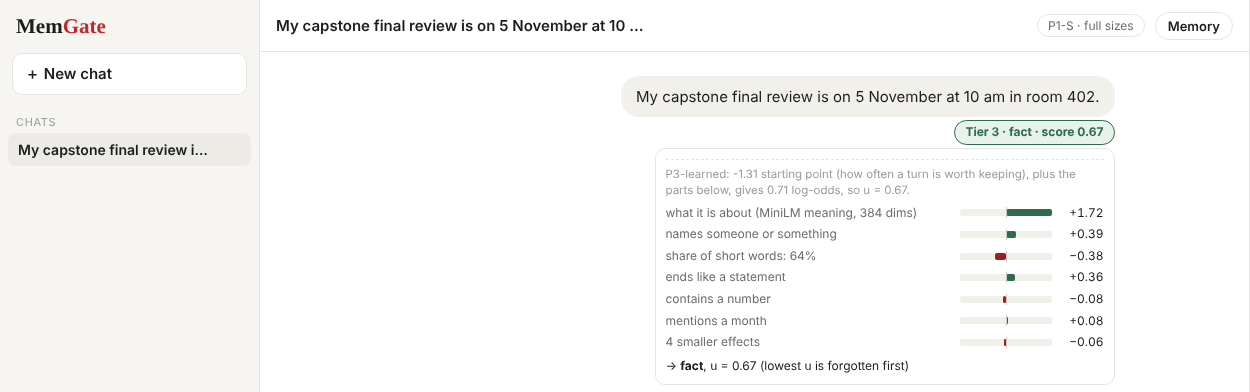
\includegraphics[width=\textwidth]{images/app_tags.png}
\caption{The application tags each message with its tier and score; the
breakdown shows why the learned scorer kept a dated fact.}
\label{fig:apptags}
\end{figure}

\begin{figure}[htbp]
\centering
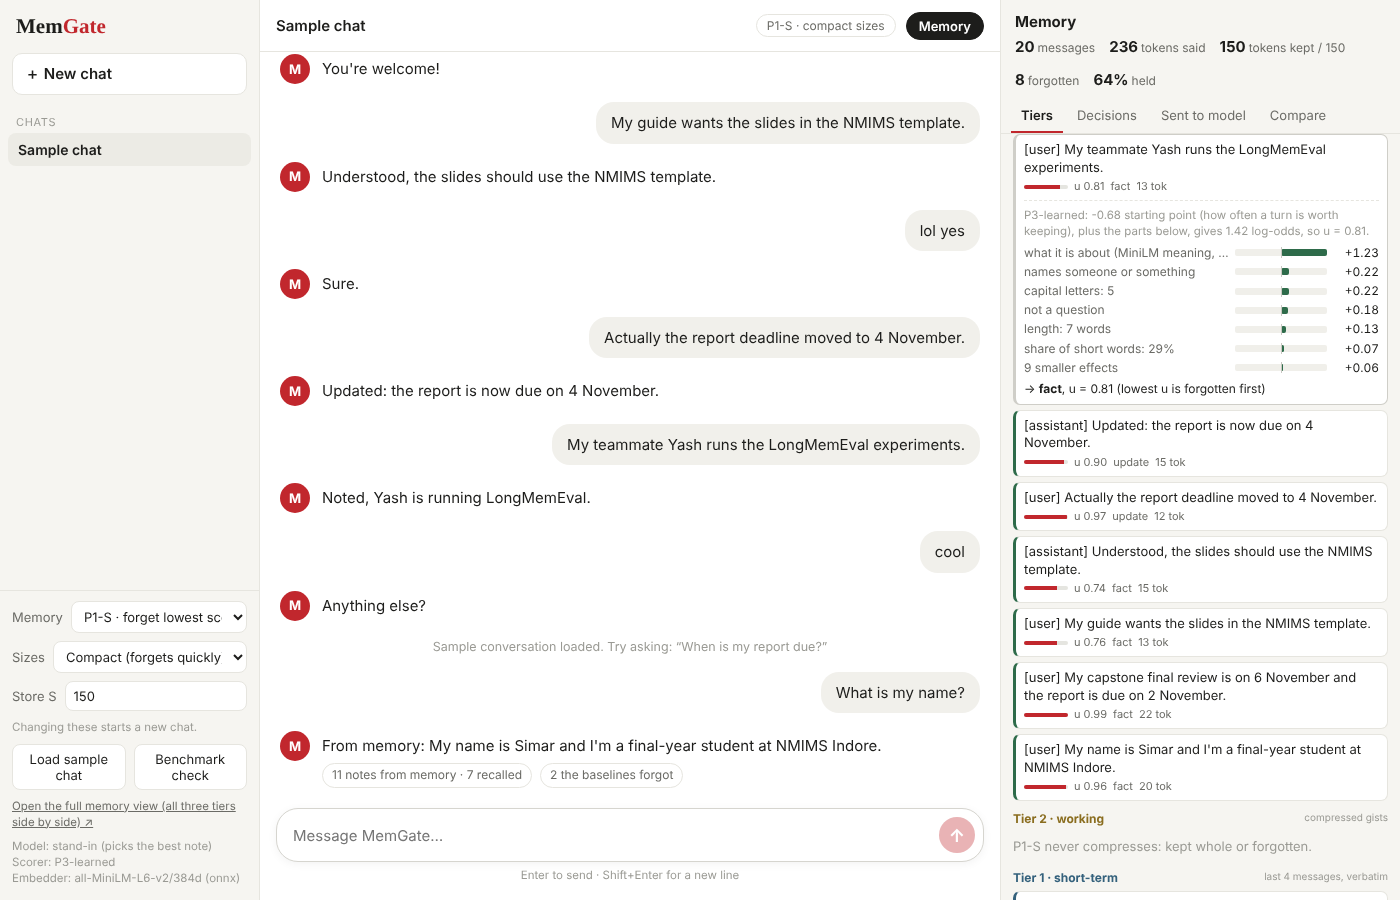
\includegraphics[width=\textwidth]{images/app_memory.png}
\caption{The memory panel: what each tier holds, with the score breakdown of
a stored note.}
\label{fig:appmemory}
\end{figure}

\begin{figure}[htbp]
\centering
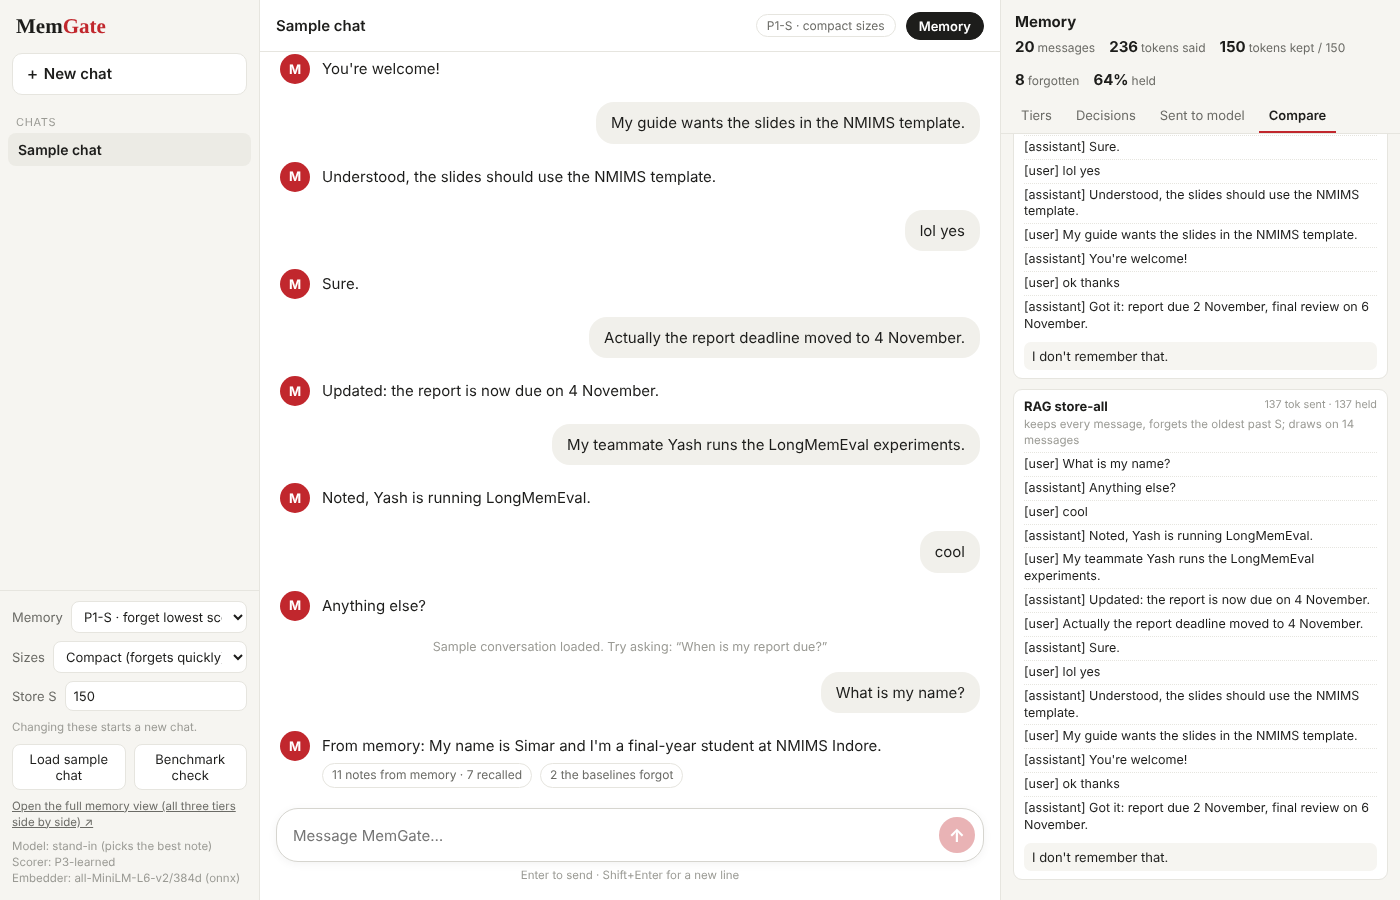
\includegraphics[width=\textwidth]{images/app_compare.png}
\caption{The Compare tab: the same question answered from MemGate, a sliding
window and RAG at the same budgets.}
\label{fig:appcompare}
\end{figure}

\begin{figure}[htbp]
\centering
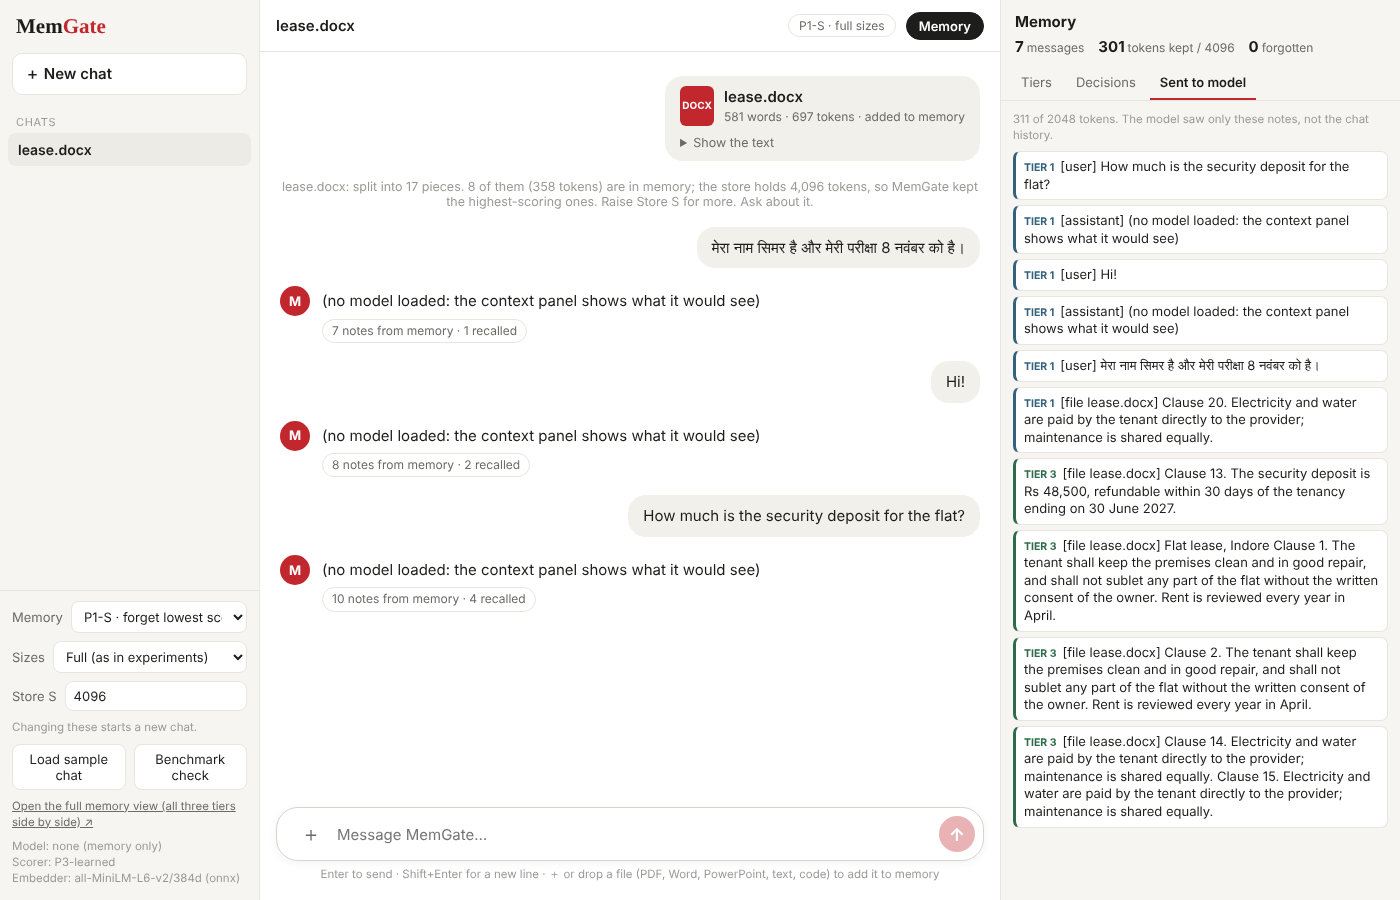
\includegraphics[width=\textwidth]{images/app_upload.png}
\caption[A Word file uploaded into a chat.]{A Word file uploaded into a chat (run without a reply model): the
file is cut into pieces, and the notes sent to the model show the recalled
clauses with their source. A Hindi message is stored the same way.}
\label{fig:appupload}
\end{figure}

\subsection{Server}
The server is a small Python standard-library HTTP server with a JSON API:
\texttt{/api/chat} sends a message, \texttt{/api/upload} adds a file,
\texttt{/api/state} returns the memory panel, \texttt{/api/why} explains a
score, \texttt{/api/rival} runs the comparison, \texttt{/api/bench} the
benchmark check, and \texttt{/api/chats/*} manages saved chats. Request bodies
are size-limited, and the accept queue was raised to 256 after a load test
(Section~\ref{sec:stress}).

\section{Testing and verification}
\label{sec:testing}
Every claim in this report is produced by a script in the repository and is
pinned by a regression test. The test suites cover the library (tiers,
compression, budgets and label-blindness), the scorers, the memory policy, the
reply models, the application endpoints, input handling, the score
explanations and comparison, the rebuilt MemGPT-style and Mem0-style
baselines, and a benchmark check that replays LoCoMo and compares it with the
published numbers. The last full run before this report passed all 453
tests. A GitHub Actions workflow runs every suite, with the real MiniLM
embedder and the LoCoMo data, on each push and pull request.

\section*{Summary}
MemGate is a pure-software memory layer with a three-tier store, a single
scoring site, a hard storage budget and a retrieval-based read path. Its
policies differ in exactly one factor each, so that the experiments isolate
one decision at a time. The learned scorer is a 399-input logistic regression
shipped as plain JSON. The same code runs a chat application that makes every
memory decision visible, and the whole system is held in place by over 450
automated tests.

\chapter{Results and Analysis}
\label{ch:results}

This chapter reports what the experiments found. Each section takes one
question, states the comparison that answers it, and gives the result with a
95\% confidence interval resampled by conversation. The chapter moves from the
accounting question (what should be budgeted), through the core decision
(select or compress), the choice of scorer and its transfer, to end-task
accuracy, comparison with existing memory designs, scale, and finally the
behaviour of the complete application. It closes with the standards that were
followed to make the results valid and reproducible. Unless stated otherwise,
the context budget is $B=2048$ tokens and answer recall is the primary metric
(Section~\ref{sec:metrics}).

\section{Storage was never budgeted}
\label{sec:accounting}

Work in this area caps the context assembled for each query and leaves the
store unbounded, and at first so did this project. Under that accounting a
store-everything baseline pays nothing to hold all 419 turns of a
conversation, so forgetting can only ever lose information. When our own
ablation was run that way, it reported the tiering and compression machinery
as a net loss against keeping everything and retrieving. Given how cost was
being counted, that verdict was correct.

A storage budget $S$ changes the question from what fits in the context to
what is worth keeping at all. Table~\ref{tab:storage} sweeps $S$ with the
context budget fixed at 2048 tokens, and the ranking under this accounting is
not the ranking under the old one. This is the most consequential observation
of the project: a protocol that leaves out a cost ends up answering a
different question from the one it seems to ask.

\section{Selection pays; compression does not}
\label{sec:selection}

Table~\ref{tab:storage} reports both metrics across the sweep, and
Fig.~\ref{fig:frontier} plots them. P1-S, which drops the lowest-utility item
when the cap binds, leads on answer recall at every budget. P1-A, which
compresses that item instead, leads on evidence recall at every budget, and
yet at $S=8192$ it falls behind even RAG on answer recall, by 3.4 points.

Here the identifier problem of Section~\ref{sec:metrics} shows up in real
numbers. A demoted gist keeps the evidence identifiers of a turn whose text is
gone. Judged on evidence recall alone, compression looks like the better use
of a bounded store; checked for whether the answer text survived, it looks
like the worse one.

\begin{table}[htbp]
\caption[Recall against the storage budget $S$ in tokens, context budget 2048.]{Recall against the storage budget $S$ in tokens, context budget 2048.
$\Delta$ is P1-S minus RAG on answer recall: identical storage, fidelity and
retrieval, differing only in which turns are forgotten.}
\label{tab:storage}
\centering
\fontsize{10}{12}\selectfont
% GENERATED by paper/make_tables.py -- do not edit by hand.
\begin{tabular}{@{}rrrrrrrr@{}}
\toprule
& \multicolumn{3}{c}{Evidence recall (\%)} & \multicolumn{3}{c}{Answer recall (\%)} & \\
\cmidrule(lr){2-4}\cmidrule(lr){5-7}
$S$ & RAG & P1-A & P1-S & RAG & P1-A & P1-S & $\Delta$ \\
\midrule
1024 & 4.3 & 9.3 & 5.3 & 9.1 & 11.9 & \textbf{15.8} & \textbf{$+6.7$} \\
2048 & 10.1 & 19.4 & 11.8 & 18.3 & 22.7 & \textbf{27.8} & \textbf{$+9.5$} \\
4096 & 17.8 & 31.8 & 20.2 & 28.1 & 30.3 & \textbf{37.5} & \textbf{$+9.4$} \\
8192 & 30.6 & 45.6 & 38.6 & 44.3 & 41.0 & \textbf{57.8} & \textbf{$+13.4$} \\
16384 & 53.3 & 58.2 & 57.9 & 66.4 & 63.1 & \textbf{71.3} & \textbf{$+4.9$} \\
\bottomrule
\end{tabular}

\end{table}

\begin{figure}[htbp]
\centering
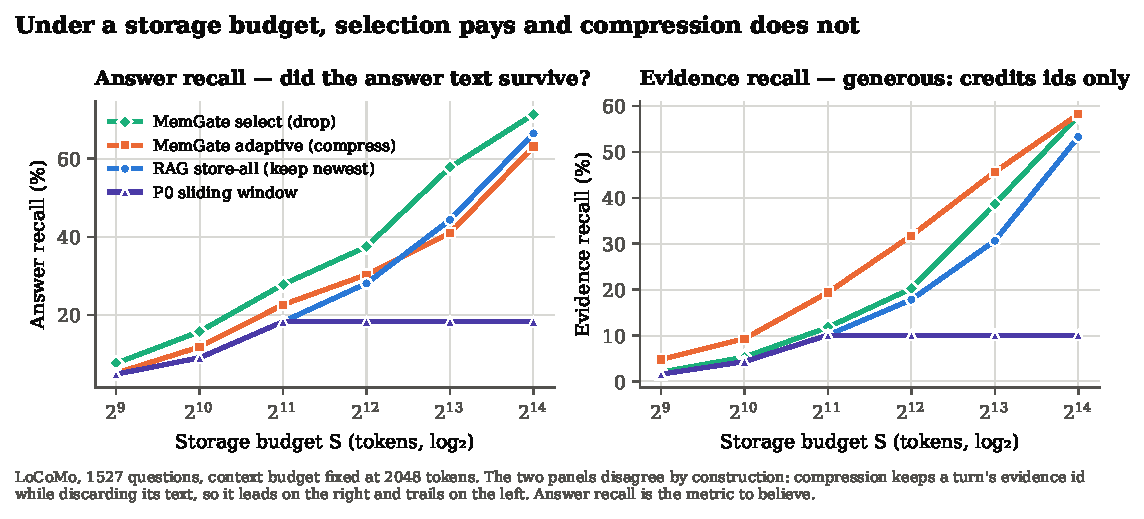
\includegraphics[width=0.85\textwidth]{../paper/figures/fig1_storage_frontier.pdf}
\caption{Recall against the storage budget for RAG, P1-A (compress) and P1-S
(drop).}
\label{fig:frontier}
\end{figure}

\section{Statistical significance}
\label{sec:significance}

Table~\ref{tab:significance} gives each contrast with intervals resampled by
conversation. Scored eviction beats FIFO on answer recall by $+9.37$ points,
and the interval excludes zero. The matching evidence-recall gain of $+2.42$
points does not survive clustering ($p=0.08$), so it is not claimed. It is
still reported, because a claim that fails a correctness check says something
useful about the check. The P1-S versus P1-A rows put signs on the divergence:
$+7.13$ on answer recall and $-11.53$ on evidence recall, both significant. The
two metrics disagree about direction, not just size.

\begin{table}[htbp]
\caption[Paired bootstrap (10{,}000 resamples) by conversation, with exact McNemar, at $S=4096$.]{Paired bootstrap (10{,}000 resamples) by conversation, with exact
McNemar, at $S=4096$. The second row is the claim we decline to make.}
\label{tab:significance}
\centering
\fontsize{10}{12}\selectfont
\begin{adjustbox}{max width=\textwidth}% GENERATED by paper/make_tables.py -- do not edit by hand.
\begin{tabular}{@{}llrcrc@{}}
\toprule
Comparison & Metric & $\Delta$ (pts) & 95\% CI (clustered) & McNemar $p$ & \\
\midrule
P1-S vs.\ RAG (FIFO) & answer & {\boldmath$+9.37$} & $[+5.45,\, +14.90]$ & $2.8\!\times\!10^{-5}$ & $\checkmark$ \\
P1-S vs.\ RAG (FIFO) & evidence & $+2.42$ & $[-1.48,\, +6.43]$ & 0.08 & \textsc{n.s.} \\
P1-S vs.\ P1-A (compress) & answer & {\boldmath$+7.13$} & $[+4.32,\, +10.28]$ & $2.1\!\times\!10^{-5}$ & $\checkmark$ \\
P1-S vs.\ P1-A (compress) & evidence & {\boldmath$-11.53$} & $[-14.73,\, -8.47]$ & $1.8\!\times\!10^{-23}$ & $\checkmark$ \\
P1-S vs.\ P0 (recency) & answer & {\boldmath$+19.16$} & $[+15.42,\, +24.13]$ & $8.2\!\times\!10^{-19}$ & $\checkmark$ \\
P1-S vs.\ P0 (recency) & evidence & {\boldmath$+10.15$} & $[+6.58,\, +13.84]$ & $1.2\!\times\!10^{-15}$ & $\checkmark$ \\
\bottomrule
\end{tabular}
\end{adjustbox}
\end{table}

\section{The rate--distortion crossover is not reached}
\label{sec:scaling}

Rate--distortion reasoning says compression must win eventually: compress a
record of everything far enough and it should beat a faithful record of only
part of it \cite{colaco2026rd}. Shrinking $S$ cannot test this, because every
policy hits the floor first, near 0.2\% evidence recall at $S=256$. The
missing axis is length, so up to ten LoCoMo conversations (186K tokens) were
concatenated with $S$ fixed, raising the compression ratio to $182\times$.
Table~\ref{tab:scaling} and Fig.~\ref{fig:scalingfig} show no crossover: the
margin of selection over compression narrows but stays positive, and the best
operating point stays at the vertex, a subset kept at full fidelity.

A concatenated stream is not a natural long conversation: each question is
about one piece and the rest act as distractors. This is therefore a stress
test of retention rather than a long-dialogue benchmark, and the crossover is
ruled out only along this axis and up to this ratio.

\begin{table}[htbp]
\caption[Answer recall (\%) against compression ratio at $S=2048$.]{Answer recall (\%) against compression ratio at $S=2048$. The last
column is the margin of dropping over compressing.}
\label{tab:scaling}
\centering
\fontsize{10}{12}\selectfont
% GENERATED by paper/make_tables.py -- do not edit by hand.
\begin{tabular}{@{}rrrrr@{}}
\toprule
Ratio & RAG & P1-A & P1-S & P1-S $-$ P1-A \\
\midrule
9$\times$ & 18.3 & 22.7 & \textbf{27.8} & $+5.2$ \\
18$\times$ & 10.8 & 13.0 & \textbf{18.9} & $+5.9$ \\
45$\times$ & 7.8 & 10.3 & \textbf{11.6} & $+1.3$ \\
91$\times$ & 4.6 & 7.4 & \textbf{8.7} & $+1.3$ \\
\bottomrule
\end{tabular}

\end{table}

\begin{figure}[htbp]
\centering
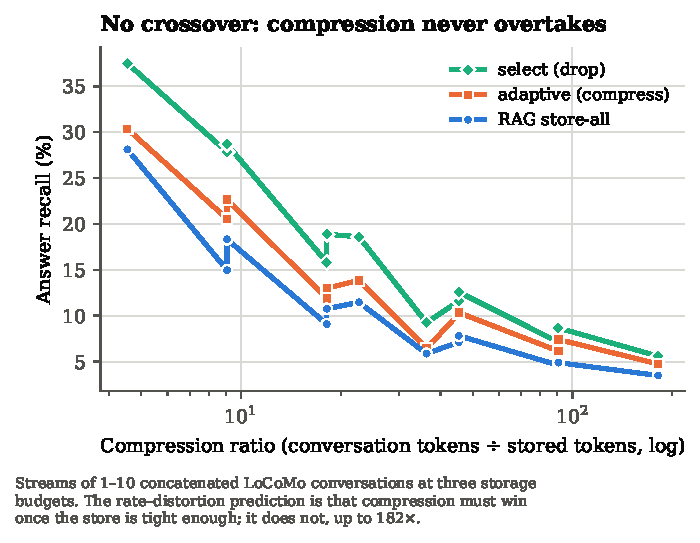
\includegraphics[width=0.85\textwidth]{../paper/figures/fig2_scaling.pdf}
\caption{Answer recall as the compression ratio grows to $182\times$.}
\label{fig:scalingfig}
\end{figure}

\section{The embedding index is not free}
\label{sec:bytes}

Counting storage in text tokens ignores the index that makes retrieval
possible. A 384-dimensional \texttt{float32} vector occupies 1{,}536\,B, while
a LoCoMo turn averages about 130\,B of text, so the index outweighs the content
it indexes by roughly a factor of 12, and the limiting resource becomes the
number of stored items rather than their length. Table~\ref{tab:cost} and
Fig.~\ref{fig:costfig} repeat the sweep with the budget in bytes and each
retrievable item charged for its vector. The selection result survives the
change of units: P1-S leads at every budget above 32\,KiB. Below about
40\,KiB, however, an embedding index cannot pay for its own storage, so P0,
which keeps no index, does best. A protocol that counts only text never sees
this regime, yet it is exactly where a memory layer on a small device would
live.

\begin{table}[htbp]
\caption[Answer recall (\%) with the budget in bytes, charging 1{,}536\,B per retrievable item for its embedding.]{Answer recall (\%) with the budget in bytes, charging 1{,}536\,B per
retrievable item for its embedding. P0 keeps no index and is flat.}
\label{tab:cost}
\centering
\fontsize{10}{12}\selectfont
% GENERATED by paper/make_tables.py -- do not edit by hand.
\begin{tabular}{@{}rrrrr@{}}
\toprule
Budget (KiB) & P0 & RAG & P1-A & P1-S \\
\midrule
32 & \textbf{18.3} & 5.0 & 5.9 & 15.1 \\
64 & 18.3 & 11.0 & 9.4 & \textbf{24.9} \\
128 & 18.3 & 20.0 & 11.9 & \textbf{33.1} \\
256 & 18.3 & 33.0 & 15.8 & \textbf{46.0} \\
512 & 18.3 & 50.3 & 22.2 & \textbf{61.0} \\
\bottomrule
\end{tabular}

\end{table}

\begin{figure}[htbp]
\centering
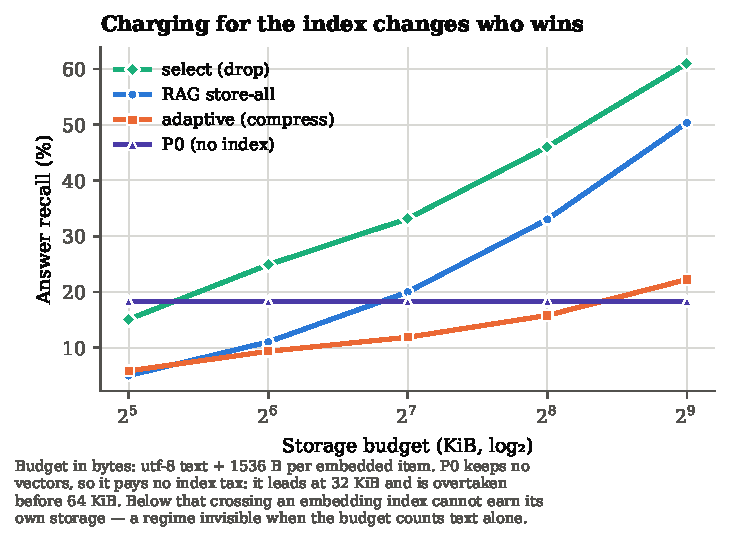
\includegraphics[width=0.85\textwidth]{../paper/figures/fig4_cost_model.pdf}
\caption{Answer recall with the storage budget counted in bytes, the index
included.}
\label{fig:costfig}
\end{figure}

\section{Scorer analysis}
\label{sec:scorer}

If the value lies in the decision, the scorer that makes it is the part worth
improving. Table~\ref{tab:ablation} removes one mechanism at a time. Retrieval
dominates, at $-31.6$ evidence points, and scored eviction is worth 6.4
points. The demotion row shows the same divergence in miniature: removing
demotion costs 11.5 evidence points and gains 7.1 answer points.

\begin{table}[htbp]
\caption[Component ablation at $S=4096$: change from the full system.]{Component ablation at $S=4096$: change from the full system.
$\dagger$: the row on which the two metrics disagree in direction.}
\label{tab:ablation}
\centering
\fontsize{10}{12}\selectfont
% GENERATED by paper/make_tables.py -- do not edit by hand.
\begin{tabular}{@{}lrr@{}}
\toprule
Component removed & $\Delta$ evidence & $\Delta$ answer \\
\midrule
Retrieval (Tier 3) & $-31.6$ & $-28.0$ \\
Demotion on pressure\,$\dagger$ & $-11.5$ & $+7.1$ \\
Scored eviction ($\rightarrow$ FIFO) & $-6.4$ & $-7.4$ \\
Informative compressor & $-4.4$ & $-1.7$ \\
Consolidation merge & $-3.4$ & $-4.8$ \\
Semantic supersession & $-0.3$ & $-0.3$ \\
\bottomrule
\end{tabular}

\end{table}

Table~\ref{tab:scorers} and Fig.~\ref{fig:scorerfig} vary only the scorer.
Three results follow, all significant under clustering. Scoring is worth
doing: the hand-written heuristic gains $+11.19$ answer points over unscored
recency. The LLM judge \cite{zheng2023judge}, however, loses: Qwen2.5-0.5B
reaches 30.9\% against the heuristic's 36.8\%, $-5.87$ points with the
interval excluding zero, at about fifteen minutes of GPU time per corpus
against microseconds for a regular expression. And the headroom is real: a
logistic scorer fitted leave-one-conversation-out reaches 48.3\%, $+11.47$
over the heuristic.

The judge fails because of what it is shown. It rates each turn on its own,
but salience is not a property of a turn on its own: a phone number matters
because someone asks for it later. The fitted scorer sees the same isolated
text but absorbs corpus-level base rates that a per-turn prompt cannot
convey; its strongest single feature is turn length, ahead of every
hand-designed cue.

\begin{table}[htbp]
\caption[Single-component scorer swap at $S=4096$.]{Single-component scorer swap at $S=4096$. Policy, retrieval and
compression fixed; only the scorer varies. P3 is fitted on the other nine
conversations. Run before the scorer fix (Section~\ref{sec:prefix}).}
\label{tab:scorers}
\centering
\fontsize{10}{12}\selectfont
\begin{adjustbox}{max width=\textwidth}\input{../paper/tables/scorers}\end{adjustbox}
\end{table}

\begin{figure}[htbp]
\centering
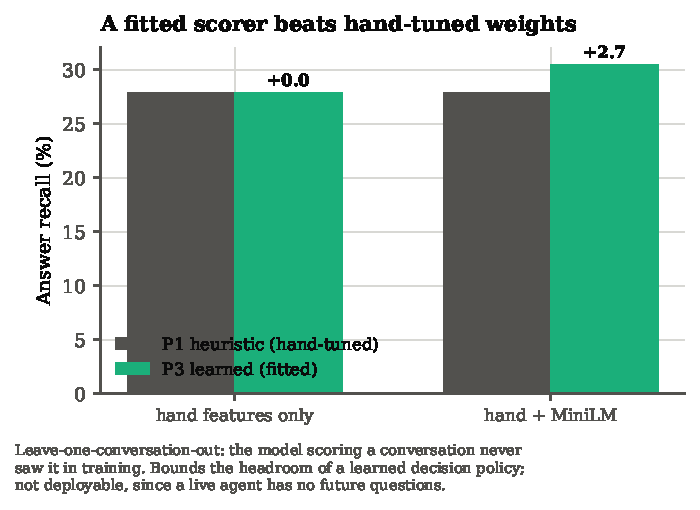
\includegraphics[width=0.8\textwidth]{../paper/figures/fig3_scorer.pdf}
\caption{Answer recall by scorer: recency, heuristic, LLM judge and learned.}
\label{fig:scorerfig}
\end{figure}

\section{A learned scorer across two corpora}
\label{sec:transfer}

LoCoMo's dialogues are generated by an LLM, so a scorer fitted to them may
learn the generator's style rather than what people later ask about. This was
tested on REALTALK \cite{lee2025realtalk}: ten conversations between real
people over 21 days, 8{,}944 turns and 660 questions, of which 160 are
answer-recoverable. Every held-out conversation is scored by three models
that never saw it: trained on the other conversations of the same corpus, on
the other corpus only, or on all 19 other conversations pooled.

Table~\ref{tab:transfer} reports the result. On LoCoMo the pooled scorer
reaches 52.0\% answer recall against the heuristic's 37.5\%, a gain of
$+14.55$ points, and pooling beats same-corpus training by $+3.36$, so adding
a different corpus helped rather than diluted. Transfer works in one
direction only. Trained on REALTALK alone, the scorer still beats the
heuristic on LoCoMo by $+9.09$; trained on LoCoMo alone, it falls below the
heuristic on REALTALK ($-4.38$, n.s.) and is significantly worse than
same-corpus training there.

Because $S=4096$ is the budget of the headline comparison rather than one
chosen for this scorer, Table~\ref{tab:transfer-budget} repeats the pooled run
at four other budgets. On LoCoMo the gain is significant from $S=2048$ to
16384 and largest at 4096. On REALTALK it is significant at $S=8192$
($+16.88$) and 16384. The embedding is what carries across: with the hand
features alone, the pooled scorer is significantly worse than the heuristic on
REALTALK ($-8.75$), because its feature weights encode LoCoMo's style. Logistic
regression was kept after comparing it with boosted trees and a 64-unit MLP:
neither beat it by more than the spread between held-out conversations, and
the trees were much slower.

\begin{table}[htbp]
\caption[Learned scorer on held-out conversations of two corpora, $S=4096$.]{Learned scorer on held-out conversations of two corpora, $S=4096$.
$\Delta$ is answer recall against P1 with 95\% intervals by conversation; bold
excludes zero.}
\label{tab:transfer}
\centering
\fontsize{10}{12}\selectfont
\begin{adjustbox}{max width=\textwidth}% GENERATED by paper/make_tables.py -- do not edit by hand.
\begin{tabular}{@{}lrrrrc@{}}
\toprule
Scorer (trained on) & AUC & Evid. & Ans. & $\Delta$ vs.\ P1 & 95\% CI \\
\midrule
\multicolumn{6}{@{}l}{\emph{LoCoMo} (715 answer-recoverable questions)} \\
\quad RAG (FIFO, no scorer) & -- & 17.8 & 28.1 & --- & --- \\
\quad P1 heuristic & 0.599 & 20.2 & 37.5 & --- & --- \\
\quad P3, same corpus & 0.793 & 32.9 & 48.7 & {\boldmath$+11.19$} & $[+4.72,\, +17.06]$ \\
\quad P3, other corpus only & 0.692 & 30.1 & 46.6 & {\boldmath$+9.09$} & $[+4.53,\, +13.46]$ \\
\quad P3, pooled (shipped) & 0.791 & 34.0 & 52.0 & {\boldmath$+14.55$} & $[+10.40,\, +19.70]$ \\
\multicolumn{6}{@{}l}{\emph{REALTALK} (160 answer-recoverable questions)} \\
\quad RAG (FIFO, no scorer) & -- & 10.5 & 16.9 & --- & --- \\
\quad P1 heuristic & 0.624 & 12.6 & 32.5 & --- & --- \\
\quad P3, same corpus & 0.737 & 18.5 & 38.8 & $+6.25$ & $[-3.01,\, +13.42]$ \\
\quad P3, other corpus only & 0.681 & 11.2 & 28.1 & $-4.38$ & $[-12.50,\, 0.00]$ \\
\quad P3, pooled (shipped) & 0.749 & 17.3 & 36.2 & $+3.75$ & $[-2.92,\, +8.65]$ \\
\bottomrule
\end{tabular}
\end{adjustbox}
\end{table}

\begin{table}[htbp]
\caption[The pooled learned scorer (P3) against the P1 heuristic across the store budget $S$, answer recall (\%).]{The pooled learned scorer (P3) against the P1 heuristic across the
store budget $S$, answer recall (\%). Bold excludes zero.}
\label{tab:transfer-budget}
\centering
\fontsize{10}{12}\selectfont
\begin{adjustbox}{max width=\textwidth}% GENERATED by paper/make_tables.py -- do not edit by hand.
\begin{tabular}{@{}rrrlrrl@{}}
\toprule
& \multicolumn{3}{c}{LoCoMo} & \multicolumn{3}{c}{REALTALK} \\
\cmidrule(lr){2-4}\cmidrule(l){5-7}
$S$ & P1 & P3 & $\Delta$ [95\% CI] & P1 & P3 & $\Delta$ [95\% CI] \\
\midrule
1024 & 15.8 & 19.0 & $+3.22$ $[0.00,\, +6.40]$ & 8.1 & 10.0 & $+1.88$ $[-1.95,\, +5.36]$ \\
2048 & 27.8 & 33.7 & {\boldmath$+5.87$} $[+1.83,\, +9.88]$ & 16.2 & 15.0 & $-1.25$ $[-10.62,\, +3.98]$ \\
4096 & 37.5 & 52.0 & {\boldmath$+14.55$} $[+10.40,\, +19.70]$ & 32.5 & 36.2 & $+3.75$ $[-2.92,\, +8.65]$ \\
8192 & 57.8 & 69.1 & {\boldmath$+11.33$} $[+6.06,\, +16.41]$ & 41.2 & 58.1 & {\boldmath$+16.88$} $[+6.31,\, +26.72]$ \\
16384 & 71.3 & 77.2 & {\boldmath$+5.87$} $[+2.04,\, +10.56]$ & 61.3 & 68.1 & {\boldmath$+6.88$} $[+2.12,\, +12.21]$ \\
\bottomrule
\end{tabular}
\end{adjustbox}
\end{table}

\section{A negative result on LongMemEval}
\label{sec:lme}

The headline was also tested on LongMemEval \cite{wu2024longmemeval}: 94
independent histories of 38--62 sessions each, with the store budget swept so
that LongMemEval was held at LoCoMo's retention (22.1\% against 22.0\%). Here
the heuristic P1-S \emph{loses} to FIFO by 21.0 answer points (95\% CI
$[-33.9,-8.1]$), where LoCoMo gives a gain. The cause is the scorer rather than
the mechanism: the heuristic's separation between evidence and non-evidence
turns reverses sign, from $+0.0476$ on LoCoMo to $-0.0346$ on LongMemEval, so
eviction discards evidence first. The heuristic was written for LoCoMo's
short dialogue lines, and LongMemEval's turns are long prose. An obvious
confound, the share of the context reserved for recent turns, was ruled out:
removing it changed answer recall by exactly zero. This run used the
heuristic before the scorer fix; the learned scorer has not yet been tested on
LongMemEval, and that is listed as future work.

\section{End-task accuracy}
\label{sec:endtask}

Everything so far is context recall, which caps end-task accuracy without
measuring it. To measure it, each assembled context was passed to one fixed
reader, Qwen2.5-1.5B-Instruct-4bit decoding greedily for at most 32 tokens,
and the output was scored with the same normaliser the answer-recall metric
uses, over all 715 answer-recoverable questions, with a closed-book arm (no
memory) and an oracle arm (exactly the cited evidence).

Table~\ref{tab:endtask} and Fig.~\ref{fig:endtask} report the outcome. The
closed-book floor is 1.7\%, so the margin above it is due to the memory layer.
P1-S reaches 18.5\% against RAG's 12.4\%, a realised gap of $+6.0$ points
(95\% CI $[+3.3,+9.1]$), which is 69\% of the $+8.7$-point recall gap between
the same two arms in this run. Accuracy given that the answer was present is
49.4\% for P1-S against 42.3\% for RAG, so P1-S both places the answer in
context more often and assembles contexts the reader uses more successfully.
The oracle converts a complete context into a correct answer 67.3\% of the
time, which locates the remaining headroom in the reader rather than in the
memory layer.

\begin{table}[htbp]
\caption[End-task accuracy through one fixed reader at $S=4096$ over all 715 answer-recoverable questions.]{End-task accuracy through one fixed reader at $S=4096$ over all 715
answer-recoverable questions. Acc.$\mid$present is accuracy on the questions
whose answer reached the context. Run before the scorer fix.}
\label{tab:endtask}
\centering
\fontsize{10}{12}\selectfont
\input{../paper/tables/endtask}
\end{table}

\begin{figure}[htbp]
\centering
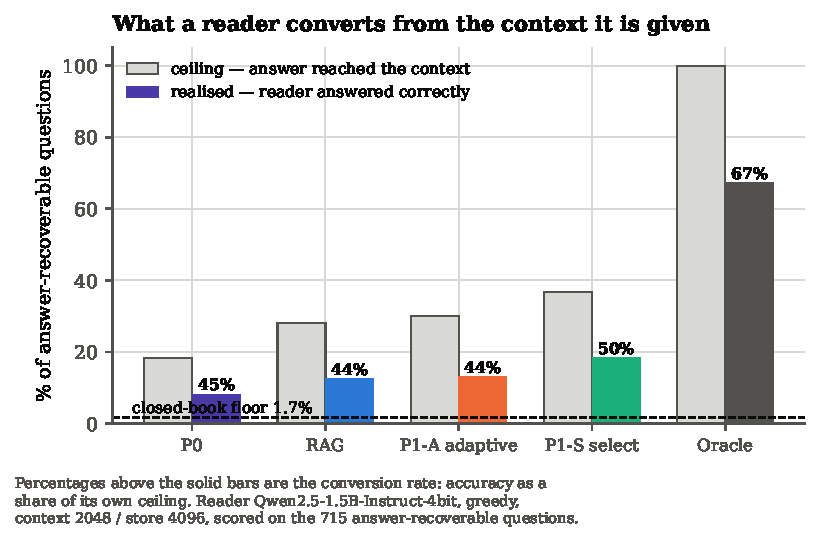
\includegraphics[width=0.8\textwidth]{../paper/figures/fig5_endtask.pdf}
\caption{Reader accuracy by memory policy, with the closed-book floor and the
oracle ceiling.}
\label{fig:endtask}
\end{figure}

Two further runs refine the compression result. Replacing the extractive
compressor with the 1.5B model rewriting each evicted turn gains $+4.06$
answer points over extractive compression (95\% CI $[+0.84,+6.66]$), so part
of the compression loss was the compressor; dropping still wins, 36.8\%
against 34.1\%, at about 1{,}850 times the compute. A scorer learned online
from retrieval feedback, with no labels and no future questions, is
statistically level with the heuristic ($-2.94$, CI $[-7.93,+1.13]$).

\section{Against MemGPT-style and Mem0-style memory}
\label{sec:external}

To compare MemGate with designs in actual use, the memory management of
MemGPT \cite{packer2023memgpt} and Mem0 \cite{chhikara2025mem0} was rebuilt
inside the same harness at the same budgets. The MemGPT-style arm keeps a
recent queue and a searchable archive and folds evicted messages into a
recursive summary that is always in context. The Mem0-style arm writes one
compressed fact per turn with ADD, UPDATE and NOOP and evicts the least
recently touched fact. Neither calls an LLM, so these are the systems' memory
structures rather than their prompts. In the baselines' favour, their
settings were grid-searched on LoCoMo itself at $S=4096$; no MemGate arm was
tuned on these answers.

Table~\ref{tab:external} and Fig.~\ref{fig:external} report the result. The
learned scorer beats both rebuilds at every budget, by $+7.3$ to $+24.6$ points
over Mem0-style and $+11.5$ to $+22.7$ over MemGPT-style, every gap significant.
The untrained P1 heuristic beats MemGPT-style everywhere but loses to the tuned
Mem0-style at $S=4096$, the budget its settings were chosen on. Mem0-style
stops improving at 52.6\% from $S=8192$, because UPDATE replaces a fact with its
nearest neighbour and so discards distinct facts that merely look alike.
MemGPT-style stays within about two points of plain RAG, because its summary
holds gists whose answers were compressed away.

\begin{table}[htbp]
\caption[Answer recall (\%) on LoCoMo against rebuilt MemGPT-style and Mem0-style memory.]{Answer recall (\%) on LoCoMo against rebuilt MemGPT-style and
Mem0-style memory. Bold $\Delta$: the interval by conversation excludes zero.}
\label{tab:external}
\centering
\fontsize{10}{12}\selectfont
\begin{adjustbox}{max width=\textwidth}% GENERATED by paper/make_tables.py -- do not edit by hand.
\begin{tabular}{@{}rrrrrrrr@{}}
\toprule
& & MemGPT & Mem0 & & & \multicolumn{2}{c}{$\Delta$ vs.\ Mem0-style} \\
\cmidrule(l){7-8}
$S$ & RAG & -style & -style & P1-S & P3 & P1-S & P3 \\
\midrule
2048 & 18.3 & 18.7 & 26.4 & 27.8 & \textbf{33.7} & $+1.4$ & {\boldmath$+7.3$} \\
4096 & 28.1 & 30.2 & 44.5 & 37.5 & \textbf{52.0} & {\boldmath$-7.0$} & {\boldmath$+7.6$} \\
8192 & 44.3 & 46.4 & 52.6 & 57.8 & \textbf{69.1} & $+5.2$ & {\boldmath$+16.5$} \\
16384 & 66.4 & 65.7 & 52.6 & 71.3 & \textbf{77.2} & {\boldmath$+18.7$} & {\boldmath$+24.6$} \\
\bottomrule
\end{tabular}
\end{adjustbox}
\end{table}

\begin{figure}[htbp]
\centering
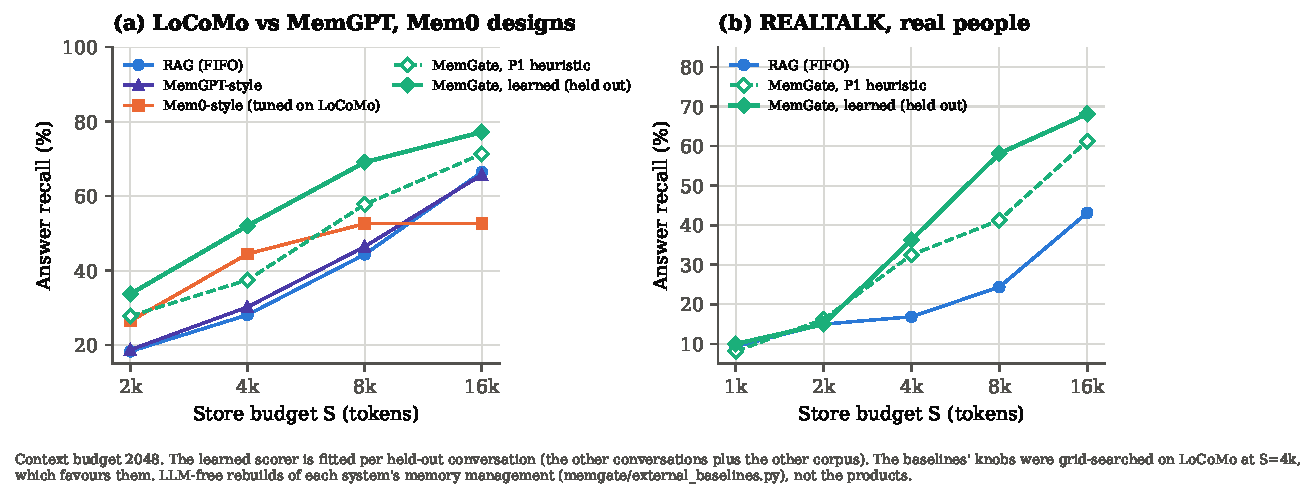
\includegraphics[width=0.8\textwidth]{../paper/figures/fig6_external.pdf}
\caption{Answer recall against the store budget for MemGate and the rebuilt
MemGPT-style and Mem0-style memories.}
\label{fig:external}
\end{figure}

\section{Chats of up to ten million tokens}
\label{sec:scale}

LoCoMo conversations average about 19K tokens. BEAM \cite{tavakoli2026beam}
supplies user--assistant chats of 100K, 500K, 1M and 10M tokens, and MemBench
\cite{tan2025membench} short agent trajectories. Each conversation was scored
by a learned scorer fitted, under five folds by conversation, without it;
BEAM 1M and 10M lie outside its training corpora altogether. The store budget
for BEAM is $S=26{,}000$, about 2.5\% of a 1M-token chat.

Table~\ref{tab:scale} reports answer recall. The learned scorer beats RAG on
all seven corpora with the interval excluding zero, by $+36.5$ points on BEAM
1M and $+46.2$ on BEAM 10M. On a million-token chat RAG keeps only the most
recent turns, so almost nothing it is asked about survives. The one corpus on
which the learned scorer is not the best is MemBench, whose short factual
statements are what the P1 rules were written to find. BEAM answers are mostly
paraphrases, so only a few questions per corpus are answer-recoverable, and
the BEAM 10M row rests on 13 questions.

\begin{table}[htbp]
\caption[Held-out answer recall (\%) at each corpus's store budget, 5-fold by conversation.]{Held-out answer recall (\%) at each corpus's store budget, 5-fold by
conversation. P3$_{12}$: the earlier recipe; P3$_{\mathrm{ship}}$: the shipped
ensemble. Bold: the interval excludes zero. $^\ddagger$PersonaChat validation
dialogues, never trained on.}
\label{tab:scale}
\centering
\fontsize{10}{12}\selectfont
\begin{adjustbox}{max width=\textwidth}% GENERATED by paper/make_tables.py -- do not edit by hand.
\begin{tabular}{@{}lrrrrrlrl@{}}
\toprule
Corpus & $S$ & $n$ & RAG & P1 & P3$_{12}$ & P3$_{12}-$RAG [95\% CI] & P3$_{\mathrm{ship}}$ & P3$_{\mathrm{ship}}-$P3$_{12}$ [95\% CI] \\
\midrule
LoCoMo & 4096 & 715 & 28.1 & 37.5 & 50.3 & {\boldmath$+22.2$} $[+17.5,\, +27.6]$ & 51.9 & $+1.5$ $[-0.2,\, +3.4]$ \\
REALTALK & 4096 & 160 & 16.9 & 32.5 & 36.2 & {\boldmath$+19.4$} $[+7.5,\, +26.4]$ & 36.2 & $0.0$ $[-3.3,\, +3.1]$ \\
BEAM 100K & 26K & 34 & 32.4 & 35.3 & 73.5 & {\boldmath$+41.2$} $[+14.3,\, +67.6]$ & 73.5 & $0.0$ $[0.0,\, 0.0]$ \\
BEAM 500K & 26K & 55 & 32.7 & 32.7 & 63.6 & {\boldmath$+30.9$} $[+16.7,\, +44.8]$ & 61.8 & $-1.8$ $[-10.0,\, +5.8]$ \\
BEAM 1M & 26K & 52 & 13.5 & 11.5 & 50.0 & {\boldmath$+36.5$} $[+21.8,\, +51.0]$ & 50.0 & $0.0$ $[-7.3,\, +8.0]$ \\
BEAM 10M & 26K & 13 & 7.7 & 23.1 & 53.8 & {\boldmath$+46.2$} $[+10.0,\, +76.9]$ & 38.5 & $-15.4$ $[-44.4,\, 0.0]$ \\
MemBench & 2048 & 367 & 76.8 & 97.5 & 95.6 & {\boldmath$+18.8$} $[+14.2,\, +23.7]$ & 97.5 & {\boldmath$+1.9$} $[+0.3,\, +3.8]$ \\
Everyday chat$^\ddagger$ & 1024 & 1762 & 28.8 & 30.4 & 61.4 & --- & 69.0 & {\boldmath$+7.6$} $[+5.9,\, +9.5]$ \\
\bottomrule
\end{tabular}
\end{adjustbox}
\end{table}

\section{Ten times the training data}
\label{sec:retrain}

The scorer that the application first shipped was fitted on 58{,}616 turns.
It was retrained on ten times that, adding BEAM 1M and 10M and MemBench,
594{,}000 turns in all. Each candidate was replayed on held-out conversations
at three to five budgets per corpus, with the folds dealt in three different
orders, 26{,}444 replays in all, under the rule that a shipped model must lose
nowhere.

More data on its own did not help (Table~\ref{tab:retrain}, first column). The
10$\times$ model gained on MemBench but lost evidence recall on BEAM 1M and
500K in every shuffle. A linear model on 399 inputs was short of capacity, not
of data, and the new turns were mostly negatives. Boosted trees, the obvious
source of capacity, lost 8.5 points on LoCoMo and were rejected. Three changes
put it right: weighting corpora within a family by their evidence turns,
adding everyday chat from PersonaChat \cite{zhang2018personachat} as a fifth
family (262{,}876 turns), and averaging the result in logit space with the
earlier model, Eq.~(\ref{eq:ens}). The shipped model is trained on 856{,}876
turns, 14.6 times the original, and has no significant loss on any corpus at
the paper's budgets; it gains $+7.6$ to $+8.2$ answer points on everyday chat.

\begin{table}[htbp]
\caption[Retraining: change against the earlier recipe in three reshuffled fold orders, held out.]{Retraining: change against the earlier recipe in three reshuffled
fold orders, held out. ``App path'' adds the application's chunking, guard
and multi-query retrieval. Bold: the interval excludes zero.}
\label{tab:retrain}
\centering
\fontsize{10}{12}\selectfont
\begin{adjustbox}{max width=\textwidth}% GENERATED by paper/make_tables.py -- do not edit by hand.
\begin{tabular}{@{}llll@{}}
\toprule
& 10x (594K turns) & \multicolumn{2}{c}{Shipped (857K turns)} \\
\cmidrule(lr){2-2}\cmidrule(l){3-4}
Corpus & Evidence & Answer & Evidence \\
\midrule
LoCoMo & $-0.4$, $-0.8$, $-0.2$ & $+1.5$, $-0.3$, $+0.3$ & $+0.1$, $-0.2$, $+0.2$ \\
REALTALK & $+0.1$, $-1.6$, $0.0$ & $0.0$, $0.0$, $+0.6$ & $-0.3$, $-0.8$, $+0.2$ \\
BEAM 100K & $-1.3$, $-0.8$, {\boldmath$-3.7$} & $0.0$, $+2.9$, $-2.9$ & $+1.8$, {\boldmath$+1.8$}, $+0.6$ \\
BEAM 500K & {\boldmath$-5.2$}, {\boldmath$-4.4$}, {\boldmath$-3.0$} & $-1.8$, $+1.8$, $+1.8$ & $+1.6$, $+2.0$, {\boldmath$+2.8$} \\
BEAM 1M & {\boldmath$-5.1$}, {\boldmath$-5.6$}, {\boldmath$-5.3$} & $0.0$, $-1.9$, $+1.9$ & $+0.3$, $0.0$, $-0.4$ \\
BEAM 10M & {\boldmath$-2.3$}, $-2.5$, $-0.5$ & $-15.4$, $0.0$, $-7.7$ & $-1.2$, $-1.8$, $+1.2$ \\
MemBench & {\boldmath$+5.5$}, {\boldmath$+5.8$}, {\boldmath$+6.2$} & {\boldmath$+1.9$}, {\boldmath$+1.9$}, {\boldmath$+2.2$} & {\boldmath$+5.6$}, {\boldmath$+5.9$}, {\boldmath$+6.4$} \\
Everyday chat$^\ddagger$ & --- & {\boldmath$+7.6$}, {\boldmath$+8.2$}, {\boldmath$+8.0$} & {\boldmath$+8.8$}, {\boldmath$+9.1$}, {\boldmath$+9.3$} \\
App path, BEAM 100K & {\boldmath$+6.1$}, $+4.2$, $+6.0$ & {\boldmath$+11.8$}, {\boldmath$+11.8$}, $+8.8$ & {\boldmath$+12.4$}, {\boldmath$+11.5$}, {\boldmath$+11.9$} \\
App path, LoCoMo & $-0.5$, $-0.7$, $-0.2$ & $+1.5$, $0.0$, $+0.4$ & $+0.3$, $+0.1$, $+0.5$ \\
App path, REALTALK & $+0.7$, $+0.3$, $-0.3$ & $+3.1$, $+1.9$, $+0.6$ & $+0.5$, $-0.1$, $0.0$ \\
\bottomrule
\end{tabular}
\end{adjustbox}
\end{table}

\section{Stress and scale through the application}
\label{sec:stress}

The complete pipeline was also tested the way a user meets it. Whole BEAM
chats were typed into the application one message at a time, exactly as its
page sends them, at $S=26{,}000$, and each answerable question was then asked
as a message. Table~\ref{tab:appbeam} reports the result: on million-token
chats, which MemGate holds at about 2.5\%, the answer reaches the reader for
51.9\% of questions against 19.2\% for RAG and 9.6\% for a sliding window. The
store never exceeded $S$, and a message took 0.49\,s on average on a shared
4-core machine.

\begin{table}[htbp]
\caption{Whole BEAM chats typed into the application one message at a time,
$S=26{,}000$; answer recall (\%).}
\label{tab:appbeam}
\centering
\fontsize{10}{12}\selectfont
\begin{adjustbox}{max width=\textwidth}% GENERATED by paper/make_tables.py -- do not edit by hand.
\begin{tabular}{@{}lrrrrrrlr@{}}
\toprule
Chats & $N$ & M tok. & $n$ & P0 & RAG & MemGate & $\Delta$ vs.\ RAG [95\% CI] & McNemar $p$ \\
\midrule
BEAM 1M & 33 & 1.07 & 52 & 9.6 & 19.2 & \textbf{51.9} & {\boldmath$+32.7$} $[+19.2,\, +46.3]$ & $9.1\!\times\!10^{-4}$ \\
BEAM 500K & 33 & 0.52 & 55 & 12.7 & 30.9 & \textbf{65.5} & {\boldmath$+34.5$} $[+19.6,\, +49.1]$ & $3.1\!\times\!10^{-4}$ \\
\bottomrule
\end{tabular}
\end{adjustbox}
\end{table}

Much of the gap comes down to where the evidence sits (Table~\ref{tab:age}).
RAG forgets oldest first, so for evidence in the first third of a
conversation it keeps the answer 8--9\% of the time; the untrained heuristic
keeps 20--33\%, and the learned scorer more. For evidence in the last third
RAG is competitive, since recency is then the right rule.

\begin{table}[htbp]
\caption[Answer recall (\%) by the position of a question's evidence, $S=4096$.]{Answer recall (\%) by the position of a question's evidence,
$S=4096$. $^\ast$In-sample on both corpora.}
\label{tab:age}
\centering
\fontsize{10}{12}\selectfont
% GENERATED by paper/make_tables.py -- do not edit by hand.
\begin{tabular}{@{}llrrrr@{}}
\toprule
Corpus & Evidence in & $n$ & RAG & P1 & P3$^\ast$ \\
\midrule
LoCoMo & first & 262 & 9.2 & 33.2 & 51.9 \\
 & middle & 225 & 14.2 & 38.2 & 53.8 \\
 & last & 228 & 63.6 & 41.7 & 54.4 \\
\midrule
REALTALK & first & 86 & 8.1 & 19.8 & 33.7 \\
 & middle & 45 & 11.1 & 40.0 & 55.6 \\
 & last & 29 & 51.7 & 58.6 & 65.5 \\
\bottomrule
\end{tabular}

\end{table}

People rarely ask one clean question per message. When each LoCoMo question
was buried in 150--450 words of other chat, using the whole message as the
query dropped answer recall from 53.1\% to 30.3\%; making each question its
own query with interleaved rankings recovers 49.8\%.

The same tests found six input-handling bugs, each now pinned by a test:
half of an emoji in one message made every later save of that chat fail; a
300\,KB Word file that unzips to 300\,MB used 3.8\,GB of memory; deeply nested
JSON dropped the connection; request bodies had no size limit; a message of
only invisible characters was accepted; and a locked PDF gave an unclear
error. A load test found one more: under bursts, the server's accept queue of
five reset 314 of 2{,}000 requests from 200 simultaneous visitors. With a queue
of 256 the same test completes with no errors in 25\,s, and a single chat of
5{,}000 messages stays at 4{,}093 of its 4{,}096 tokens, at 0.12\,s per message.

\section{Standards followed}
\label{sec:standards}

The following standards and practices were adhered to in building and
testing the system and in validating its results.
\begin{itemize}
\item \textbf{IEEE Std 754 (floating-point arithmetic).} All embeddings and
  model weights are IEEE~754 single-precision (\texttt{float32}) values;
  the 1{,}536-byte cost of a vector in Eq.~(\ref{eq:cost}) is $384\times4$
  bytes of this format.
\item \textbf{ISO/IEC/IEEE 29119 (software testing) and IEEE Std 1012
  (verification and validation).} Testing follows their structure: unit
  tests for each module, integration tests through the application's API,
  and a benchmark-level validation test that replays LoCoMo and compares it
  with the published numbers; regression tests pin every fixed defect.
\item \textbf{ISO/IEC/IEEE 29148 (requirements engineering).} The scope,
  in-scope and out-of-scope items and the measurable objectives of
  Chapter~\ref{ch:intro} were written as verifiable requirements, each
  checked by an experiment or a test.
\item \textbf{Unicode and UTF-8 (RFC 3629).} All text is stored as UTF-8 and
  NFC-normalised; control characters, zero-width marks and bidirectional
  overrides are removed on input.
\item \textbf{RFC 9110 (HTTP semantics) and RFC 8259 (JSON).} The
  application's server uses standard HTTP methods and status codes and
  exchanges JSON.
\item \textbf{Statistical practice.} Paired bootstrap confidence intervals
  clustered by conversation \cite{efron1993bootstrap,cameron2008cluster} and
  exact McNemar tests \cite{mcnemar1947,dietterich1998tests}; a result is
  claimed only when its interval excludes zero.
\item \textbf{Reproducibility.} Every model is a pinned local copy; every
  table is generated from committed result files; and the leakage invariant
  (no decision may read an evaluation label) is enforced by tests
  \cite{kaufman2012leakage,kapoor2023leakage}.
\end{itemize}

\section*{Summary}
Once the store is bounded, deciding what to forget is worth $+9.37$ answer
points over FIFO, while compressing instead of dropping costs $7.13$; no
rate--distortion crossover appears up to $182\times$; and counting the index
in bytes reverses the ranking below about 40\,KiB. An LLM judge loses to a
heuristic, but a learned scorer beats the heuristic by $+14.55$ points on
held-out conversations, transfers from human to generated dialogue, beats
MemGPT-style and Mem0-style memory at every budget, and keeps the answer for
51.9\% of questions on million-token chats against 19.2\% for retrieval. Two
results are negative: the heuristic fails on LongMemEval, and ten times the
data alone did not improve the scorer.

\chapter{Advantages, Limitations and Applications}
\label{ch:adv}

This chapter steps back from individual results to assess MemGate as a
system: what it does better than the alternatives, where it falls short or
has not yet been tested, and where it can be applied.

\section{Advantages}
\begin{enumerate}
\item \textbf{Bounded cost on every turn.} The store never exceeds its budget
  $S$ and the prompt never exceeds $B$, however long the conversation grows.
  In the application a 5{,}000-message chat stayed at 4{,}093 of its 4{,}096
  tokens, and million-token chats were held at about 2.5\% of their length.
\item \textbf{Better recall at the same budget.} At identical storage,
  fidelity and retrieval, scored forgetting beats oldest-first forgetting by
  $+9.37$ answer points, and the learned scorer adds a further $+14.55$ over
  the heuristic on held-out conversations. It beats rebuilt MemGPT-style and
  Mem0-style memory at every budget tested.
\item \textbf{Works with any model.} The base LLM is a black box. MemGate
  needs no training of the model, so it can sit in front of a local model, a
  hosted API, or a newer model later, unchanged.
\item \textbf{Cheap to run.} Scoring a message is a 399-weight dot product
  plus one sentence embedding; there is no LLM call on the write path. The
  whole layer runs on a laptop CPU, and the shipped scorer is a small JSON
  file.
\item \textbf{Transparent decisions.} Every keep, compress and forget
  decision has a score and an explanation that a user can inspect, which an
  LLM-driven memory cannot easily offer.
\item \textbf{Measured, not asserted.} Each design choice was tested against
  a control that differs in one factor, with clustered confidence intervals,
  and the results that did not hold are reported as such.
\item \textbf{Private and offline.} With the local reply model, the memory
  and the chats stay on the user's machine and nothing needs the internet
  after setup.
\item \textbf{Robust input handling.} Long pastes, documents, other
  languages, emoji and code are cleaned, chunked and guarded before they
  reach the scorer, and the server held 200 simultaneous visitors without an
  error after the load-test fix.
\end{enumerate}

\section{Limitations}
\begin{enumerate}
\item \textbf{Context recall is not accuracy.} Most results measure whether
  the answer reached the context. End-task accuracy was measured through one
  small reader model, and that run, with the LLM-judge, abstractive and
  LongMemEval runs, was made before the scorer fix and has not been repeated.
\item \textbf{The heuristic does not transfer to every corpus.} On
  LongMemEval the hand-written scorer's separation between evidence and other
  turns reverses sign and selection loses to FIFO. The learned scorer has not
  yet been tested there.
\item \textbf{Limited statistical power on human conversation.} REALTALK has
  160 answer-recoverable questions in ten conversations, so the learned
  scorer's gains there are significant only once the store holds about 40\%
  of a conversation.
\item \textbf{Proxies in the scale tests.} BEAM answers are mostly
  paraphrases, so few questions per corpus are answer-recoverable (13 for
  BEAM 10M), and the everyday-chat test uses persona lines as queries, which
  share wording with the evidence.
\item \textbf{A linear scorer.} Logistic regression was kept because nothing
  beat it reliably, but it is short of capacity: ten times more data did not
  help on its own.
\item \textbf{Text only.} Images, audio and tool outputs that are not text
  are out of scope.
\item \textbf{One slow path.} Reopening a saved million-token chat replays it
  through memory and takes about 70\,s.
\item \textbf{Dependence on the reply model.} When the free hosted model is
  busy the application falls back to a small local model, whose answers are
  weaker even when the right notes are supplied.
\end{enumerate}

\section{Applications}
\begin{enumerate}
\item \textbf{Personal and customer-support assistants} that must remember a
  user's details, preferences and past requests across weeks without sending
  the whole history on every call.
\item \textbf{Coding and research agents} whose working history (files read,
  decisions taken, errors seen) grows far beyond the context window.
\item \textbf{On-device assistants.} The byte-level results show which
  policy to use when the memory budget is a few tens of kilobytes, as on a
  phone or an embedded device.
\item \textbf{Education and tutoring}, where a tutor should recall what a
  student has already learnt and where they struggled.
\item \textbf{Healthcare and legal intake assistants}, where specific names,
  dates and amounts must be kept while small talk can be forgotten (subject to
  the privacy rules of those domains).
\item \textbf{Document question answering} over long uploaded files, using
  the chunk, score and recall path of the application.
\item \textbf{Evaluating other memory systems.} The harness itself can be
  used to measure any memory policy against controls under a bounded store.
\end{enumerate}

\section*{Summary}
MemGate keeps cost bounded, improves recall at the same budget, works with
any model, runs cheaply and explains its decisions. Its main limitations are
that some results are measured as context recall or before the scorer fix,
that transfer to every corpus is not established, and that the scorer is
linear. It applies wherever a long-running assistant must remember specific
facts under a cost or memory limit.

\chapter{Conclusion and Future Scope}
\label{ch:concl}

This chapter summarises the work carried out, the conclusions drawn from the
results of Chapter~\ref{ch:results}, and the directions in which the work can
be taken further.

\section{Conclusion}

This project set out to measure the memory decision of an LLM agent: what to
keep, what to compress, what to forget and what to recall. It built MemGate, a
memory layer in front of a frozen model, as a harness in which each of these
decisions can be swapped and compared against a control that differs in
exactly one factor, under a store held to a fixed budget.

Under the accounting this field normally uses, tiered compression loses to
storing everything and retrieving. That result is an artefact of leaving the
store unbounded. Once the store is bounded, deciding which items to forget is
worth $+9.37$ answer-recall points at identical storage, fidelity and
retrieval, while compressing an evicted item instead of dropping it costs
$7.13$. The point at which rate--distortion theory says compression should
start to pay is not reached by $182\times$. Counting the embedding index in the
budget reverses the ranking below about 40\,KiB.

The obvious route to a better scorer, an LLM judge, loses to a regular
expression, because salience is not a property of a turn read on its own. A
logistic scorer over a sentence embedding, trained on generated and human
conversations together, beats the heuristic by $+14.55$ points on held-out
LoCoMo conversations and by a significant margin at every store budget from
2048 to 16384 tokens. It transfers from human dialogue to generated dialogue,
but not the other way round. Through a fixed reader, $+6.0$ points of the
recall advantage survive as correct answers. The same scorer beats
MemGPT-style and Mem0-style memory at every budget tried, beats retrieval on
held-out chats of up to ten million tokens, and, when million-token chats are
typed into the application, keeps the answer 51.9\% of the time against
19.2\%. Ten times the training data did not, on its own, produce a better
linear scorer; weighting corpora by their labels, adding everyday chat and
averaging with the earlier model did.

The practical advice from this work is narrow but well supported: keep a
scored subset at full fidelity rather than compressing everything, and count
the memory budget in bytes with the index included. The learned scorer ships
in a working chat application that makes every one of these decisions visible
to its user, and the findings have been written up as a research paper.

\section{Future scope}
\begin{enumerate}
\item \textbf{Re-run the pre-fix experiments.} The LLM-judge, end-task,
  abstractive and LongMemEval runs were made before the scorer fix and should
  be repeated with the fixed heuristic and the shipped learned scorer.
\item \textbf{LongMemEval with the learned scorer.} The heuristic inverts on
  LongMemEval; whether the learned scorer does too is the most important open
  test of transfer.
\item \textbf{More human-written evidence.} The learned scorer's gains on
  human conversation are significant only at larger budgets. More annotated
  human conversations, rather than a larger model, are what would settle
  this.
\item \textbf{Personalised online learning.} A scorer learned online from
  retrieval feedback is already level with the heuristic with no labels.
  Starting it from the pooled scorer and letting it adapt to each user is the
  step from a scorer fitted to benchmarks to one fitted to the person using
  the application.
\item \textbf{More capacity without losing speed.} A small non-linear scorer
  that keeps the write path cheap, tested under the same lose-nowhere rule.
\item \textbf{Multimodal memory.} Extending the tiers and the scorer to
  images, audio and tool outputs.
\item \textbf{Deployment.} Faster reopening of very long saved chats,
  multi-user hosting, and integration as a memory module for agent
  frameworks.
\end{enumerate}

\section*{Summary}
Selection beats compression under a bounded store, a learned scorer beats both
a heuristic and an LLM judge, and the result holds through a reader, against
existing memory designs and at million-token scale. The open questions are
transfer to every corpus and adaptation to each user.


\clearpage
\phantomsection
\addcontentsline{toc}{chapter}{References}
\bibliographystyle{IEEEtran}
\bibliography{../paper/refs}

\appendix
%% Appendices A-D, as listed in the guideline table of contents.

\chapter{Soft Code Flowcharts}
\label{app:flow}

This appendix gives the flowcharts of the two paths a message takes through
the MemGate application: storing it (Fig.~\ref{fig:flowwrite}) and answering
from memory (Fig.~\ref{fig:flowread}). The routing and budget loops inside the
library are shown in Fig.~\ref{fig:routing}, the scorer's guard in
Fig.~\ref{fig:scoring}, and the training of the shipped scorer in
Fig.~\ref{fig:training}.

\begin{figure}[htbp]
\centering
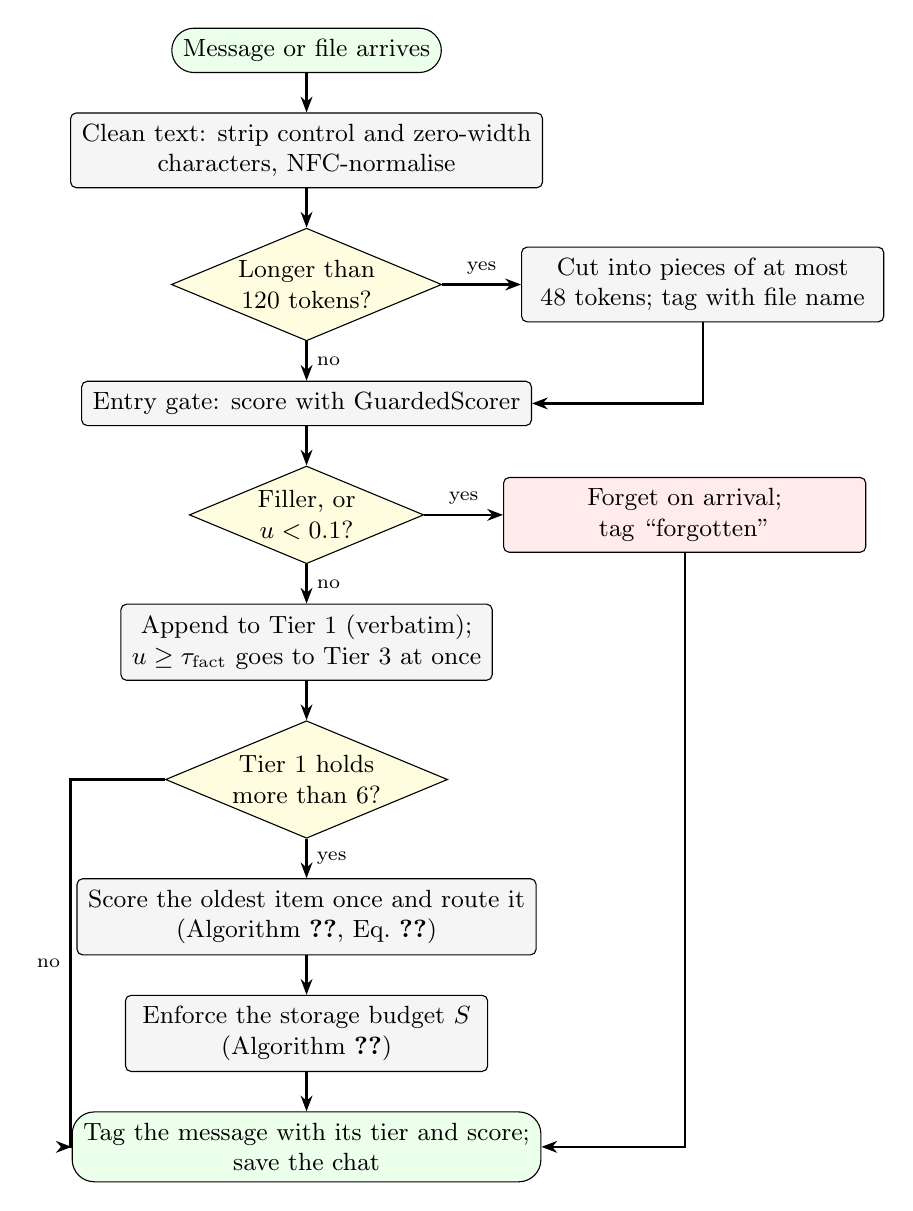
\begin{tikzpicture}[node distance=5mm and 6mm, font=\small,
  st/.style={draw, rounded corners=8pt, fill=green!8, align=center, inner sep=4pt, minimum width=3.4cm},
  pr/.style={draw, rounded corners=2pt, fill=gray!8, align=center, inner sep=4pt, minimum width=4.6cm},
  dc/.style={draw, diamond, aspect=2.4, fill=yellow!12, align=center, inner sep=1pt},
  ar/.style={->, >={Stealth[length=2mm]}, thick}]
\node[st] (in) {Message or file arrives};
\node[pr, below=of in] (clean) {Clean text: strip control and zero-width\\characters, NFC-normalise};
\node[dc, below=of clean] (long) {Longer than\\120 tokens?};
\node[pr, right=10mm of long] (chunk) {Cut into pieces of at most\\48 tokens; tag with file name};
\node[pr, below=of long] (gate) {Entry gate: score with GuardedScorer};
\node[dc, below=of gate] (fill) {Filler, or\\$u<0.1$?};
\node[pr, right=10mm of fill, fill=red!8] (forget) {Forget on arrival;\\tag ``forgotten''};
\node[pr, below=of fill] (t1) {Append to Tier 1 (verbatim);\\$u\ge\tau_{\text{fact}}$ goes to Tier 3 at once};
\node[dc, below=of t1] (full) {Tier 1 holds\\more than 6?};
\node[pr, below=of full] (route) {Score the oldest item once and route it\\(Algorithm~\ref{alg:observe}, Eq.~\ref{eq:route})};
\node[pr, below=of route] (budget) {Enforce the storage budget $S$\\(Algorithm~\ref{alg:budget})};
\node[st, below=of budget] (out) {Tag the message with its tier and score;\\save the chat};
\draw[ar] (in) -- (clean);
\draw[ar] (clean) -- (long);
\draw[ar] (long) -- node[above, font=\scriptsize]{yes} (chunk);
\draw[ar] (chunk) |- (gate);
\draw[ar] (long) -- node[right, font=\scriptsize]{no} (gate);
\draw[ar] (gate) -- (fill);
\draw[ar] (fill) -- node[above, font=\scriptsize]{yes} (forget);
\draw[ar] (fill) -- node[right, font=\scriptsize]{no} (t1);
\draw[ar] (t1) -- (full);
\draw[ar] (full) -- node[right, font=\scriptsize]{yes} (route);
\draw[ar] (route) -- (budget);
\draw[ar] (budget) -- (out);
\draw[ar] (full.west) -- ++(-12mm,0) |- node[pos=0.25, left, font=\scriptsize]{no} (out.west);
\draw[ar] (forget) |- (out.east);
\end{tikzpicture}
\caption{Flowchart of the write path in the application: how one message is
cleaned, gated, stored and kept within budget.}
\label{fig:flowwrite}
\end{figure}

\begin{figure}[htbp]
\centering
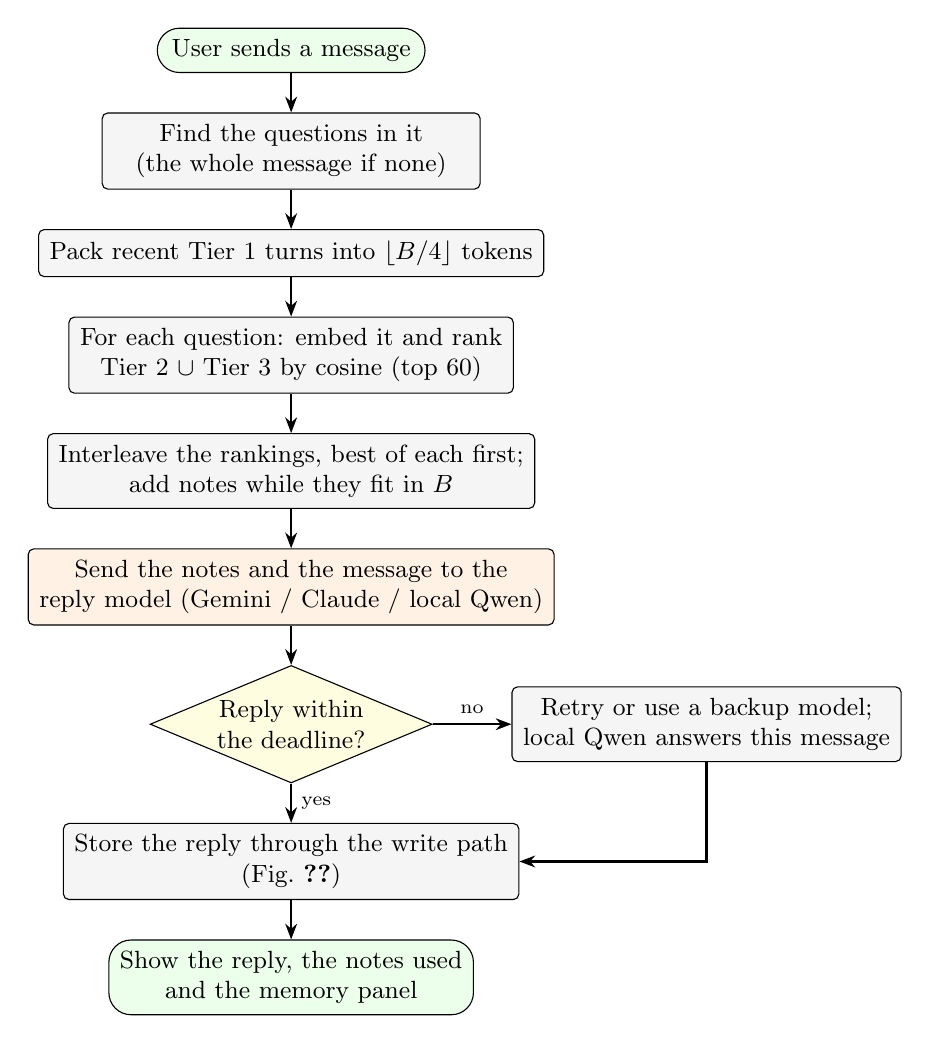
\begin{tikzpicture}[node distance=5mm and 6mm, font=\small,
  st/.style={draw, rounded corners=8pt, fill=green!8, align=center, inner sep=4pt, minimum width=3.4cm},
  pr/.style={draw, rounded corners=2pt, fill=gray!8, align=center, inner sep=4pt, minimum width=4.8cm},
  dc/.style={draw, diamond, aspect=2.4, fill=yellow!12, align=center, inner sep=1pt},
  ar/.style={->, >={Stealth[length=2mm]}, thick}]
\node[st] (in) {User sends a message};
\node[pr, below=of in] (q) {Find the questions in it\\(the whole message if none)};
\node[pr, below=of q] (t1) {Pack recent Tier 1 turns into $\lfloor B/4\rfloor$ tokens};
\node[pr, below=of t1] (ret) {For each question: embed it and rank\\Tier 2 $\cup$ Tier 3 by cosine (top 60)};
\node[pr, below=of ret] (mix) {Interleave the rankings, best of each first;\\add notes while they fit in $B$};
\node[pr, below=of mix, fill=orange!10] (llm) {Send the notes and the message to the\\reply model (Gemini / Claude / local Qwen)};
\node[dc, below=of llm] (ok) {Reply within\\the deadline?};
\node[pr, right=10mm of ok] (fb) {Retry or use a backup model;\\local Qwen answers this message};
\node[pr, below=of ok] (obs) {Store the reply through the write path\\(Fig.~\ref{fig:flowwrite})};
\node[st, below=of obs] (out) {Show the reply, the notes used\\and the memory panel};
\draw[ar] (in) -- (q);
\draw[ar] (q) -- (t1);
\draw[ar] (t1) -- (ret);
\draw[ar] (ret) -- (mix);
\draw[ar] (mix) -- (llm);
\draw[ar] (llm) -- (ok);
\draw[ar] (ok) -- node[above, font=\scriptsize]{no} (fb);
\draw[ar] (fb) |- (obs);
\draw[ar] (ok) -- node[right, font=\scriptsize]{yes} (obs);
\draw[ar] (obs) -- (out);
\end{tikzpicture}
\caption{Flowchart of the read path in the application: how a reply is
assembled from memory.}
\label{fig:flowread}
\end{figure}

\chapter{Data Sheets}
\label{app:data}

MemGate uses no hardware components, so its data sheets describe the datasets
and models it depends on (Tables~\ref{tab:datasets} and~\ref{tab:models}). All
datasets are public and were used under their published licences; no personal
data was collected by the project.

\begin{table}[htbp]
\caption{Datasets used.}
\label{tab:datasets}
\centering
\fontsize{9}{11}\selectfont
\begin{tabularx}{\textwidth}{@{}>{\raggedright\arraybackslash}p{2.8cm}>{\raggedright\arraybackslash}p{4.4cm}>{\raggedright\arraybackslash}X@{}}
\toprule
\textbf{Dataset} & \textbf{Size} & \textbf{Use in this project} \\
\midrule
LoCoMo \cite{maharana2024locomo} & 10 conversations, 5{,}882 turns, 1{,}527 questions (715 answer-recoverable) & Main benchmark; LLM-generated multi-session dialogue with marked evidence \\
REALTALK \cite{lee2025realtalk} & 10 conversations, 8{,}944 turns, 660 questions (160 answer-recoverable) & Human conversation over 21 days; transfer test and training \\
BEAM 100K / 500K \cite{tavakoli2026beam} & 20 and 35 chats & Long user--assistant chats; training and held-out tests \\
BEAM 1M & 35 chats, 74{,}630 turns, 622 questions with evidence & Held-out million-token test; app-path test \\
BEAM 10M & 10 chats, 208{,}696 turns, 128 pinned questions & Held-out ten-million-token test \\
MemBench \cite{tan2025membench} & 4{,}330 trajectories, 252{,}058 turns & Short factual agent memories; training and test \\
PersonaChat \cite{zhang2018personachat} & 894 long chats (262{,}876 turns) train; 50 chats test & Everyday chat with weak labels from persona lines \\
LongMemEval \cite{wu2024longmemeval} & 94 histories of 38--62 sessions & Second-benchmark test of the headline \\
\bottomrule
\end{tabularx}
\end{table}

\begin{table}[htbp]
\caption{Models and tokeniser used.}
\label{tab:models}
\centering
\fontsize{9}{11}\selectfont
\begin{tabularx}{\textwidth}{@{}>{\raggedright\arraybackslash}p{3.8cm}>{\raggedright\arraybackslash}p{3.6cm}>{\raggedright\arraybackslash}X@{}}
\toprule
\textbf{Model} & \textbf{Size} & \textbf{Role} \\
\midrule
all-MiniLM-L6-v2 \cite{reimers2019sbert,wang2020minilm} & 22.7M parameters, 384-d output, about 90\,MB & Embeddings for retrieval, dedupe, supersession and the learned scorer \\
Learned scorer P3 (this work) & 399 weights + bias, plain JSON & Utility of each message \\
Qwen2.5-0.5B-Instruct \cite{qwen2025} & 0.5B parameters & LLM judge of salience (P2) \\
Qwen2.5-1.5B-Instruct \cite{qwen2025} & 1.5B parameters (4-bit on Apple silicon) & End-task reader; abstractive compressor; offline reply model \\
Google Gemini (flash) \cite{gemini2023} & hosted & Default reply model in the application (free key) \\
\texttt{cl100k\_base} (tiktoken) & 100K-token vocabulary & Exact token counts for every budget \\
\bottomrule
\end{tabularx}
\end{table}

\chapter{List of Components}
\label{app:components}

MemGate has no hardware components. Its software components are listed in
Tables~\ref{tab:files} and~\ref{tab:libs}. The source code is in the
project repository (branch \texttt{endtask-full-run}).

\begin{table}[htbp]
\caption{Software components: main files of the repository.}
\label{tab:files}
\centering
\fontsize{9}{11}\selectfont
\begin{tabularx}{\textwidth}{@{}>{\raggedright\arraybackslash}p{6.4cm}>{\raggedright\arraybackslash}X@{}}
\toprule
\textbf{File or folder} & \textbf{Purpose} \\
\midrule
\texttt{memgate/memgate/} & The library (Table~\ref{tab:modules}) \\
\texttt{memgate/app.py}, \texttt{web/chat.html} & The chat application: server and page \\
\texttt{run\_locomo.py},\newline \texttt{run\_storage\_sweep.py} & LoCoMo evaluation and the storage-budget sweep \\
\texttt{run\_ablations.py}, \texttt{run\_significance.py} & Component ablations; bootstrap and McNemar tests \\
\texttt{run\_scaling.py}, \texttt{run\_cost\_model.py} & Compression-ratio scaling; byte accounting \\
\texttt{train\_scorer.py}, \texttt{train\_transfer.py},\newline \texttt{retrain\_10x.py}, \texttt{export\_scorer.py} & Training, transfer tests, retraining and export of the learned scorer \\
\texttt{run\_judge\_eval.py}, \texttt{run\_endtask.py} & LLM-judge comparison; end-task accuracy \\
\texttt{run\_longmemeval.py},\newline \texttt{run\_abstractive.py}, \texttt{run\_online.py} & LongMemEval; abstractive compression; online learning \\
\texttt{run\_external\_baselines.py} & MemGPT-style and Mem0-style comparison \\
\texttt{scale\_app.py}, \texttt{stress\_inputs.py},\newline \texttt{stress\_questions.py} & Application scale, load and stress tests \\
\texttt{test\_*.py}, \texttt{run\_tests.py} & Test suites and their runner \\
\texttt{setup.sh}/\texttt{.ps1}, \texttt{start.sh}/\texttt{.bat} & One-command setup and start \\
\texttt{deploy/} & Docker image for an online Hugging Face Space \\
\texttt{paper/} & Research paper sources, generated tables and diagrams \\
\bottomrule
\end{tabularx}
\end{table}

\begin{table}[htbp]
\caption{Software libraries.}
\label{tab:libs}
\centering
\fontsize{9}{11}\selectfont
\begin{tabularx}{\textwidth}{@{}p{4.2cm}X@{}}
\toprule
\textbf{Library} & \textbf{Use} \\
\midrule
NumPy & Vectors and numerics \\
tiktoken & Token counting \\
sentence-transformers / ONNX Runtime & MiniLM embeddings \\
huggingface\_hub & One-time model downloads \\
PyTorch, Transformers, mlx-lm & Local Qwen models (judge, reader, offline replies) \\
scikit-learn & Training the learned scorer \\
Matplotlib & Figures \\
pypdf & Reading uploaded PDF files \\
anthropic (optional) & Claude replies \\
Python standard library & HTTP server, JSON, Word/PowerPoint reading, statistics \\
\bottomrule
\end{tabularx}
\end{table}

\chapter{List of Papers Presented and Published}
\label{app:papers}

The following paper was prepared from this project.

\begin{enumerate}
\item Yash Ramchandani$^{\dagger}$, Simar Singh Khanuja$^{\dagger}$ and
  Dr.\ Praveen Modi$^{*}$, ``\paperTitle''. School of Technology Management
  \& Engineering, SVKM's NMIMS, Indore Campus.
  ($^{\dagger}$equal contribution; $^{*}$corresponding author.)

  \begin{itemize}
  \item Conference version: IEEE two-column format.
  \item Journal version: single-column manuscript in the Springer Nature
    style, with a declarations section.
  \item Status: \blankfield{9cm}\\
    (venue, date of submission or acceptance, and plagiarism / AI-similarity
    report to be attached here)
  \end{itemize}
\end{enumerate}

\textbf{Abstract of the paper.} Agents built on large language models
accumulate conversations far longer than any context window, so a memory layer
must decide what to keep, compress, forget and recall. Existing memory systems
are evaluated end to end, so the value of each of these decisions on its own
is unknown. The paper presents MemGate, a harness that sits between an agent
and a frozen LLM, isolates the memory policy, and compares policies changing
one factor at a time. Once the store is bounded, choosing which turns to
forget gains $+9.37$ answer-recall points over oldest-first eviction at
identical storage, fidelity and retrieval on LoCoMo, whereas compressing
evicted turns loses $7.13$ points, with no rate--distortion crossover up to
$182\times$ compression. A logistic scorer over shallow features and a
sentence embedding beats a hand-written heuristic by $+14.55$ points on
held-out conversations, outperforms MemGPT-style and Mem0-style memory at every
budget tested, and on million-token chats typed into the application keeps the
answer for 51.9\% of questions against 19.2\%.



\end{document}
